%%%%%%%%%%%%%%%%%%%%%%%%%%%%%%%%%%%%%%%%%
% Journal Article
% LaTeX Template
% Version 1.4 (15/5/16)
%
% This template has been downloaded from:
% http://www.LaTeXTemplates.com
%
% Original author:
% Frits Wenneker (http://www.howtotex.com) with extensive modifications by
% Vel (vel@LaTeXTemplates.com)
%
% License:
% CC BY-NC-SA 3.0 (http://creativecommons.org/licenses/by-nc-sa/3.0/)
%
% Template modified by Alison Sheltong for STAT 626 Final Project.
%%%%%%%%%%%%%%%%%%%%%%%%%%%%%%%%%%%%%%%%%

%----------------------------------------------------------------------------------------
%	PACKAGES AND OTHER DOCUMENT CONFIGURATIONS
%----------------------------------------------------------------------------------------

\documentclass[twoside,twocolumn]{article}

\usepackage[greek,english]{babel} % Language hyphenation and typographical rules
\usepackage{graphicx}
\usepackage{float, enumitem}
\usepackage{amssymb,amsfonts,textcomp}
\usepackage{caption}
\usepackage{lmodern}
\usepackage{booktabs} % Horizontal rules in tables

\usepackage{hyperref} % For hyperlinks in the PDF

\usepackage{blindtext} % Package to generate dummy text throughout this template - helpful for double checking spaccing.

\usepackage[utf8x]{inputenc} %Because I like this one better than the one in the template
\usepackage{natbib}
\bibliographystyle{apalike}


\usepackage[margin=.75 in, hmarginratio=1:1,top=32mm,columnsep=20pt]{geometry} % Document margins, provided extra space for us with smaller margins than the default.

\usepackage{enumitem} % Customized lists
\setlist[itemize]{noitemsep} % Make itemize lists more compact

\usepackage{abstract} % Allows abstract customization - The italics for example.
\renewcommand{\abstractnamefont}{\normalfont\bfseries} % Set the "Abstract" text to bold
\renewcommand{\abstracttextfont}{\normalfont\small\itshape} % Set the abstract itself to small italic text

\usepackage{fancyhdr} % Headers and footers
\pagestyle{fancy} % All pages have headers and footers
\lhead{\bfseries Group 4}
\chead{\bfseries STAT 626: Time Series Analysis}
\rhead{\bfseries US Unemployment Trends} 
\lfoot{}
\cfoot{\thepage}
\rfoot{} 


\usepackage{titling} % Customizing the title section 

%----------------------------------------------------------------------------------------
%	TITLE SECTION
%----------------------------------------------------------------------------------------

\setlength{\droptitle}{-4\baselineskip} % Move the title up

\pretitle{\begin{center}\huge\bfseries} % Article title formatting
\posttitle{\end{center}} % Article title closing formatting
\title{US Unemployment Trends} % Article title
\author{%
\textsc{Joseph Blubaugh}\thanks{Plots, Data Prep, Code Management} \\[1ex] % Your name
\normalsize Statistics\\ % Your institution
%\normalsize \href{mailto:john@smith.com}{john@smith.com} % Your email address
\and % Uncomment if 2 authors are required, duplicate these 4 lines if more
\textsc{Sean Roberson}\thanks{Presentor} \\[1ex] % Second author's name
\normalsize Mathematics, Industrial\\ % Second author's institution
\and 
\textsc{Akarshan Puri}\thanks{Model selection and fitting} \\[1ex] 
\normalsize Electrical Engineering\\ 
\and 
\textsc{Alison Shelton}\thanks{Write-up} \\[1ex] 
\normalsize Statistics\\ 
\and 
\textsc{Travis Lilley}\thanks{Diagnostics} \\[1ex] 
\normalsize Statistics\\ 
\and
\textsc{Bo Pang}\thanks{Model fitting and plots} \\[1 ex]
\normalsize Psychology, Statistics
\vspace*{.5 cm}
}
%\institute[Texas A\&M] % I'm not sure yet how to add this in with the way that I put in the author names.
	%	{Texas A\&M \newline College Station, Texas}
\date{July 25, 2016 \vspace*{.25 cm}} % Final write-up due date plus a bit of extra space
\renewcommand{\maketitlehookd}{%
\begin{abstract}
\noindent The information from above is from the original presentation.  The links as to who did what should be modified probably at the end.  This is just a starting point. Also the abstract should be written last so I thought it was a good place to put this information.

\vspace*{.25 cm}
\noindent The writeup below has dummy text so I could set up the sections. I also moved some of the older write-up text to this document to start it all up.
\end{abstract}
}



%----------------------------------------------------------------------------------------

\begin{document}

% Print the title
\maketitle

%----------------------------------------------------------------------------------------
%	ARTICLE CONTENTS
%----------------------------------------------------------------------------------------

\section{Introduction}
		Unemployment has been a topic of concern throughout the United States in recent years.  The Great Recession iof 2007 was accompanied the worst unemployment crises seen since the 1930s \citep{wanberg2012individual}.   The results have been enduring, in 2010 the US job deficit was estimated to be over 10 million \citep{katz2010}. Graduate and Undergraduate college students alike are concerned over their employment prospects, wondering if their degrees will be enough to gain them a job after graduation.  These worries are well-founded as full-reovery of college graduate employment rates and earning is expected to be a slow process \cite{carnevale2015hard}.  In these times of economic uncertainty, obtaining an income generating position is not the guarantee it has seemed to be in generations past.
		
Unemployment has far-reaching consequences that extends beyond financial security. Unemployment is linked to psychological difficulties, including depression and suicide, and even physical deterioration \citep{wanberg2012individual, insecure, suicide}. A study of Greek students found a relationship between parental unemployment and PTSD symptoms related to bullying \citep{kanellopoulos2014epa}. In Nigeria, unemployment has been linked to insurgency and terrorism \citep{terrorism}. Given the impact that unemployment has on fiscal, mental, and physical health, reasearch into unemployment patterns an important part of developing policies to improve the welfare of the local, national, and global populace.

\subsection{Goal}
		The purpose of our project is to examine trends in unemployment in the United States. We will focus on the years surrounding the Great Recession of 2007, 1992 to 2015.  Our goal is to forcast unemployment into 2016. 

\subsection{Data}

The unemployment data being examined was obtained from the seasonaly adjusted, monthly, Civilian Unemployment Rate Series (UNRATE), published by the Bureau of Labor Statistics (BLS).  This series includes unemployment figures from January of 1948 to  May of 2016 \citep{blsrefsa}.  The response variable being analyzed is the unemployment rate defined as the percentage of the labor force that is unemployed.  In defining this variable, the BLS restricts this to, ``people 16 years of age and older, who currently reside in 1 of the 50 states or the District of Columbia, who do not reside in institutions (e.g., penal and mental facilities, homes for the aged), and who are not on active duty in the Armed Forces''.

Resession dates were obtained from the National Bureau of Economic Research (NBER) \citep{NBER2016}. The NBER identifies recessions and US business cycles based upon a variety of economic indicators. These include Gross Domestic Product (GDP), Gross Domestic Income (GDI), and a variety of less well known indicators such as Aggregate hours of work in the total economy.

We also explored several potential predictor variables that are potentially related to unemployment.  Industrial Production measures enterprise output of the U.S. establishments \citep{BGFS2016}. Value of Manufacturers' New Orders for All Manufacturing Industries refers to manufacturer's sales and inventory, except for New Orders from the Semicondutor Industry \citep{vmno}. The Purchase Only House Price Index for the United States follows sales for a specific set of single-family homes \citep{fhfa2016}. We also included Retailers Sales \citep{retail2016} and Total Construction Spending \citep{construction2016}.



%------------------------------------------------

\section{Exploratory Analysis}
		\begin{figure}[H]
		\centering
		\caption{Plot of the original data}
		\label{fig:unemployment}
		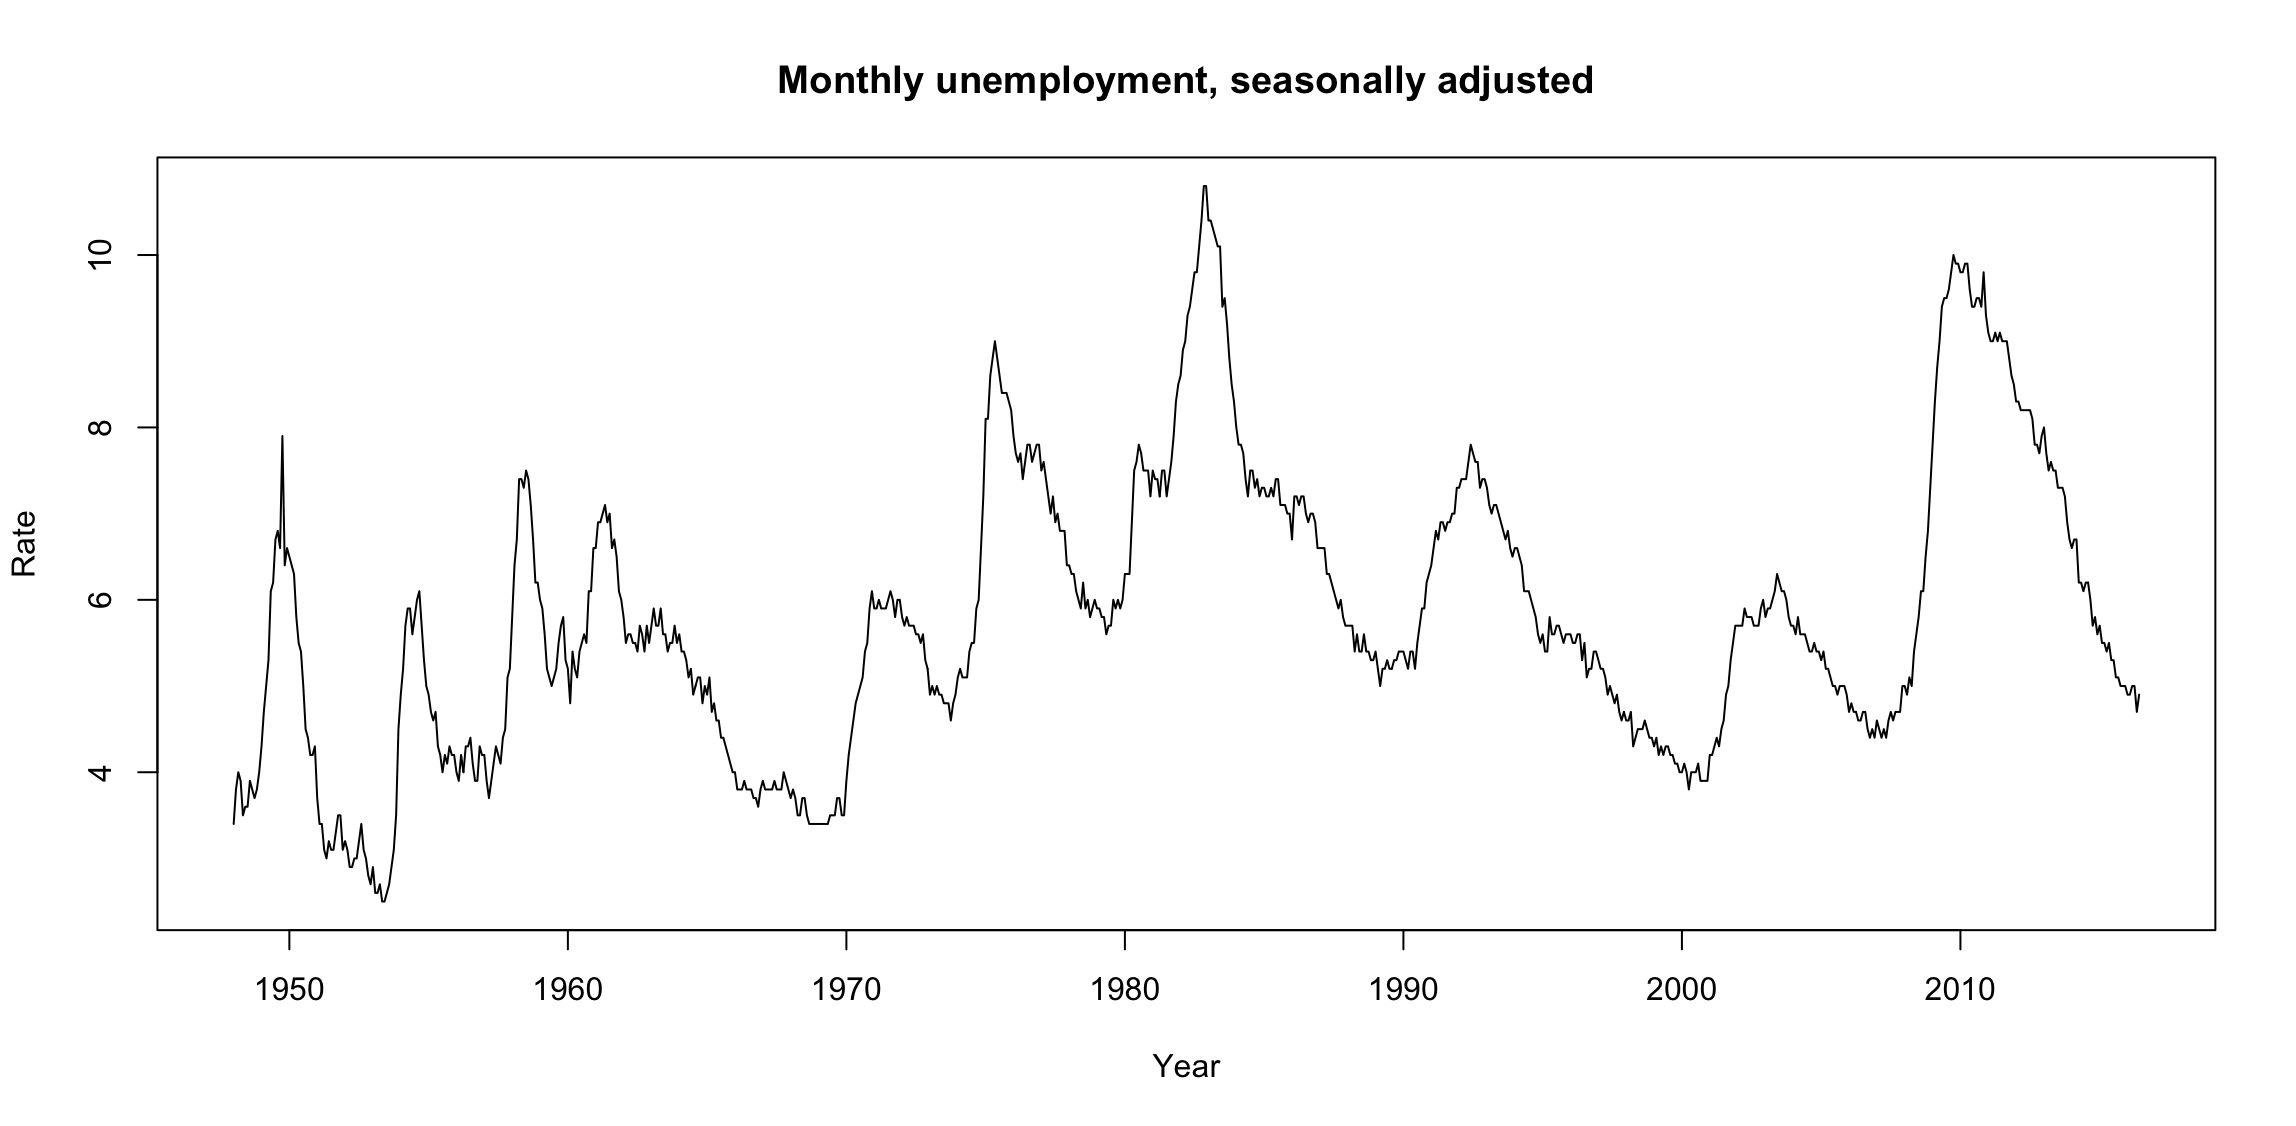
\includegraphics[width=\linewidth]{images/unemployment_total_sa}
	\end{figure}
	
			\begin{figure}[H]
		\centering
		\caption{Smoothed unemployment for the study time period}
		\label{fig:presunemp}
		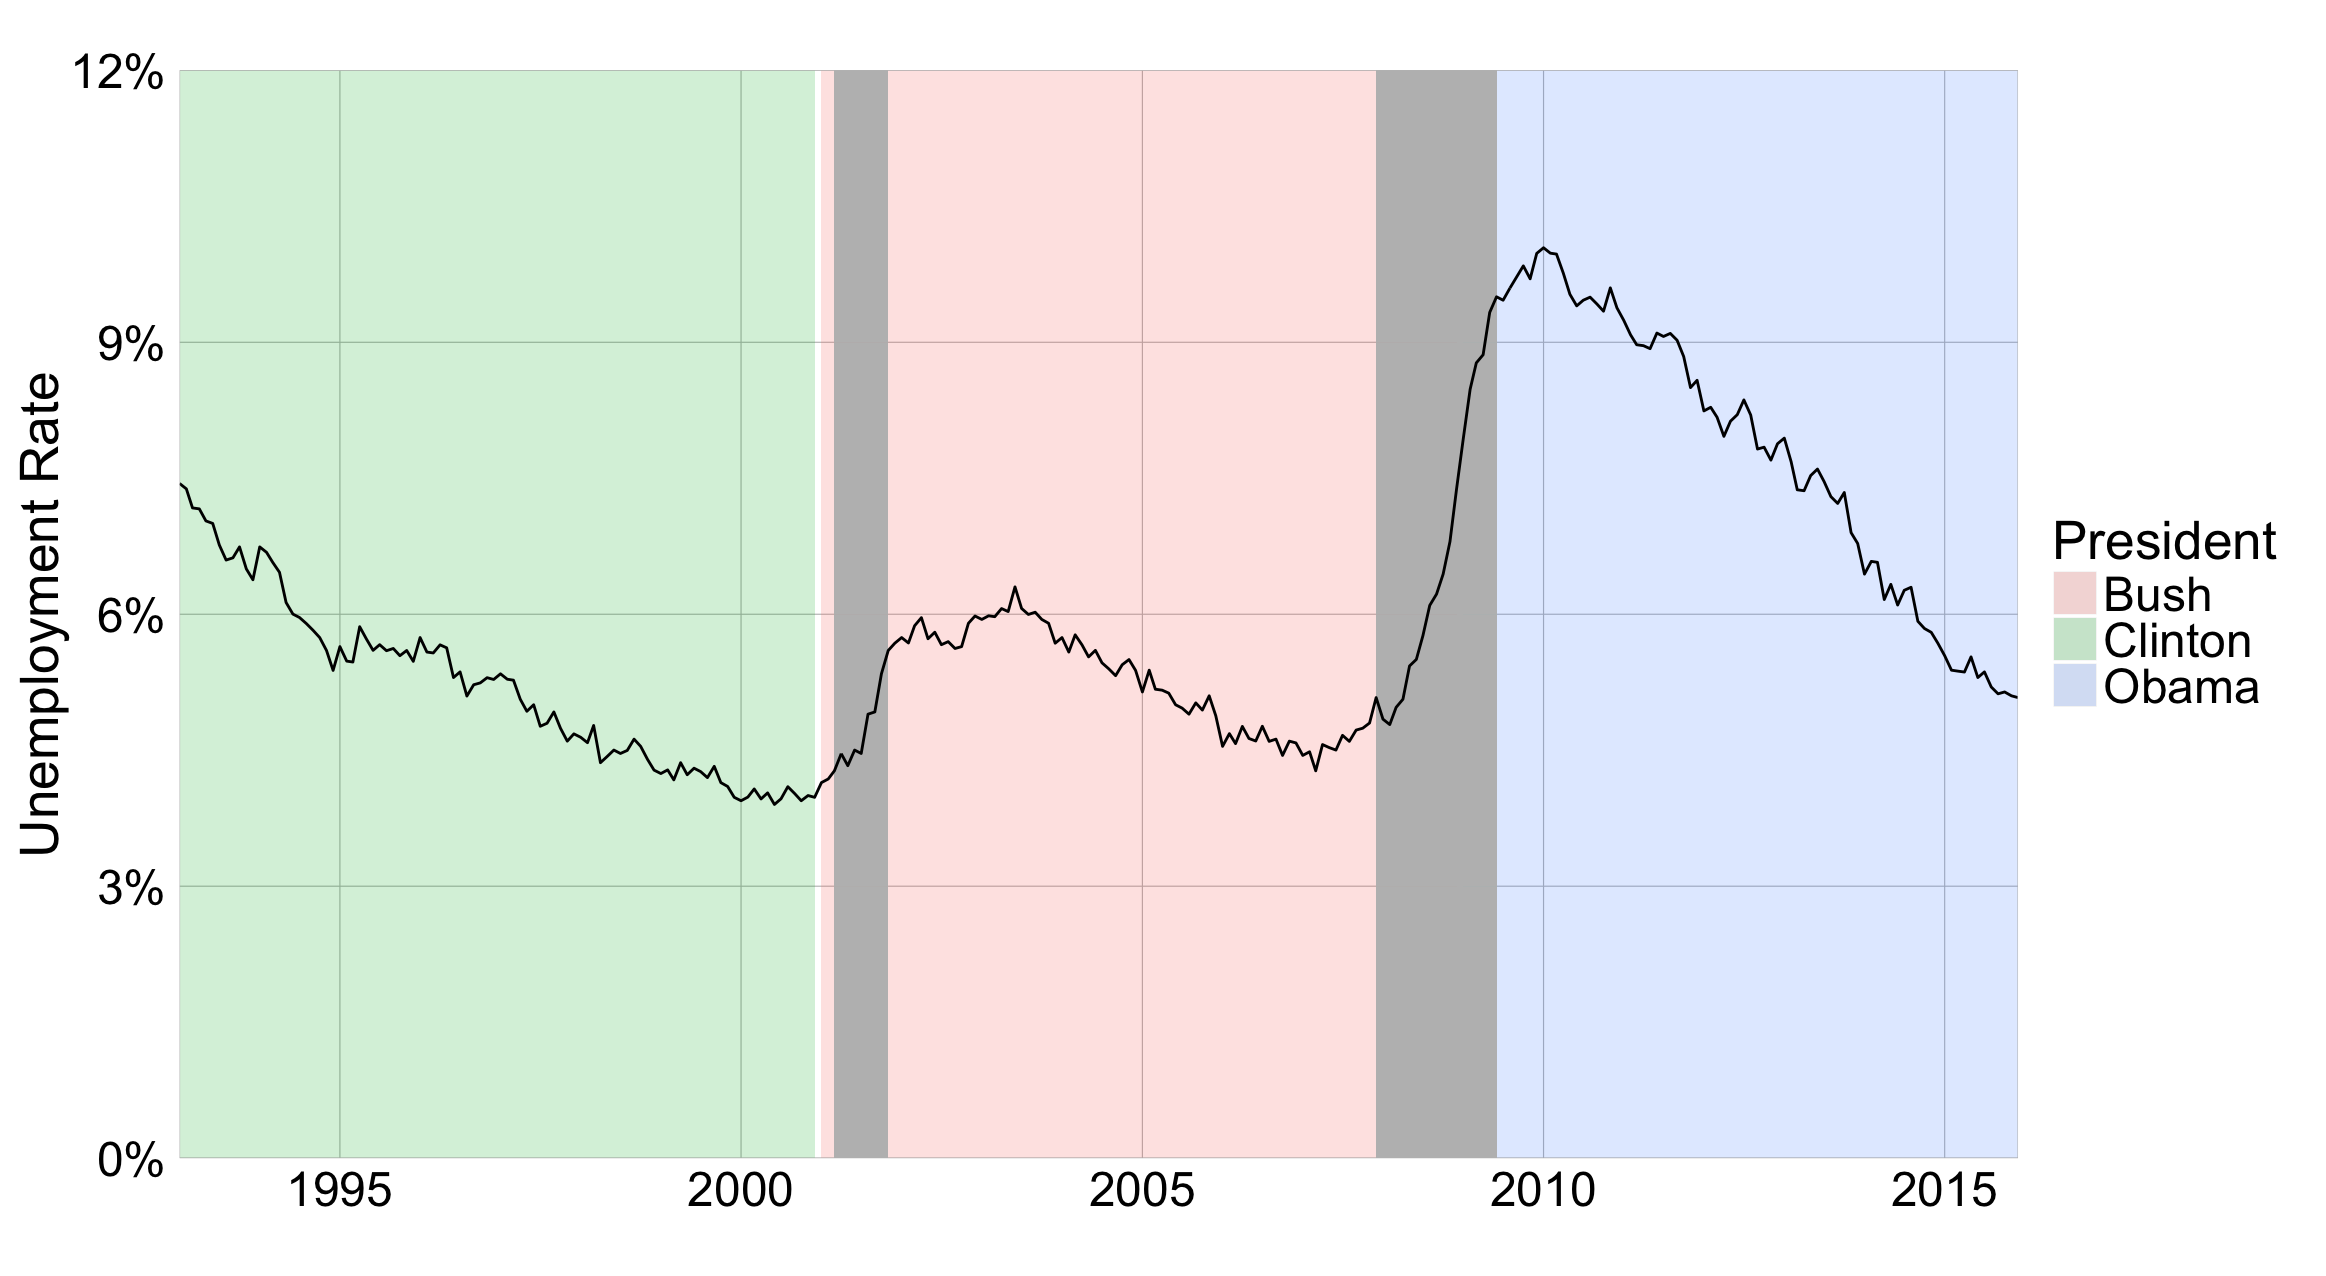
\includegraphics[width=\linewidth]{images/presunemp}
	\end{figure}


As a first step, the data was plotted over time to identify any obvious patterns visually, considering the seasonlly adjusted version of the unemployment rate, see Figure \ref{fig:unemployment}.  Overall, unemployment appears relatively volatile.  There are several time periods of sudden spikes in the unemployment rate, followed by a slower recovery period. This countercyclical movement is consistent with the descriptions of unemployment data found in the literature \citep{katz2010, Montgomery1998, shimer2012reassessing}. 

Due to marked potential differences in the trend surrounding times of economic downturn, such as those that occured after World War II and in the 70s and the 80s, we have chosen to limit our analysis on a more recent set of unemployment data. Ultimately, we decided to focus the time preceeding and following the Great Recession of 2007. We limited our inital analysis to 1992 to 2015, which encompases the presidential terms of Bill Clinton, George W. Bush, and Barack Obama, each serving eight years in office.  Initial graphs of the data seem to indicate that, in general, unemployment spiked at the begining of each president's term and fell gradually over the time he was in office, see Figure \ref{fig:presunemp}. There are also two noticeable spikes the represent that recessions of 2001 and 2008, respectively.  The 2008 recession also follows the burst of a housing market bubble.  These are all explanatory variables that can potentially inform unemployment patterns. A scatterplot of these predictors can be seen in Figure \ref{fig:pred_scatt}.

			\begin{figure}[H]
		\centering
		\caption{Scatterplot of unemployment and potential predictors}
		\label{fig:pred_scatt}
		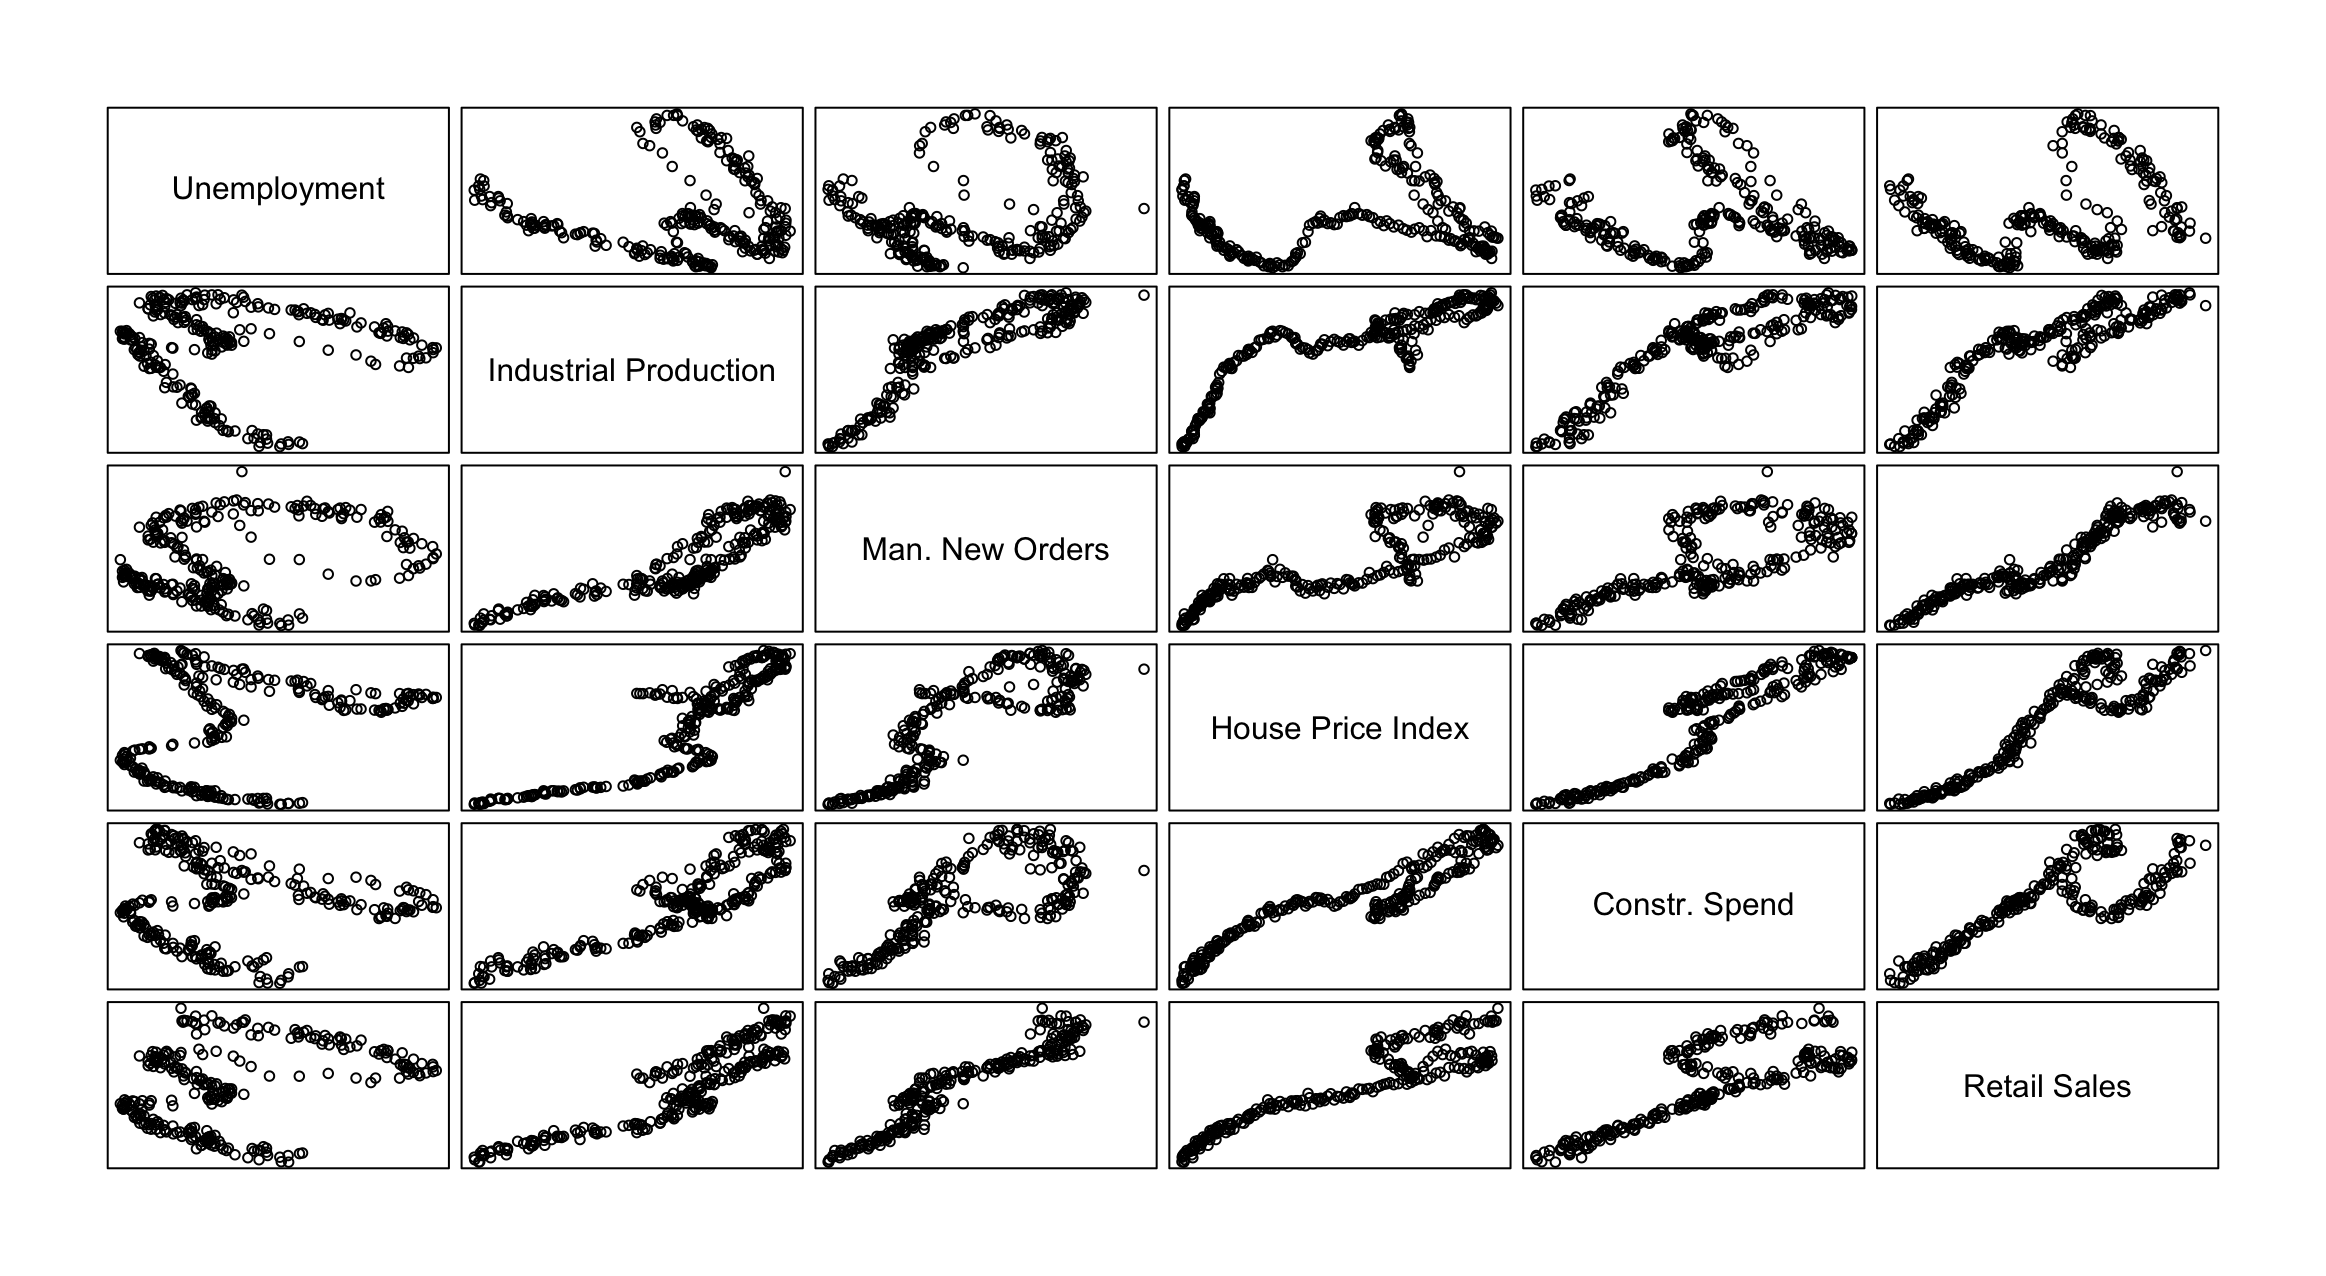
\includegraphics[width=\linewidth]{images/pred_scatt}
	\end{figure}
	

%Text requiring further explanation\footnote{Example footnote}. I don't think we need footnotes

%------------------------------------------------

\section{Achieving Stationarity}

In analyzing the inital plots, it appears that the series could benefit from detrending. A graph of various potential lagged values for unemployment can be seen in Figure \ref{fig:laggedunemployment}. The high values of the correlation coffecients, particularly through lag 6 further suggest a high degree of autocorrelation within the unemployment dataset.    An Augmented Dickey-Fuller (ADF) test for stationarity was conducted to verify the nonstationarity of the unemployment data.  The ADF test tests the null hypothesis that the time series data has a unit root against the alternative that the data are stationary \citep{Shumway2006}. The Dickey-Fuller test statistic for the unemployment data is -2.1377, with a lag order of 6, and a p-value of 0.518. The high p-values suggest that we do not have a stationary model with just the raw unemployment data.
			
						\begin{figure}[H]
		\centering
		\caption{Autocorrelation of unemployment data}
		\label{fig:laggedunemployment}
		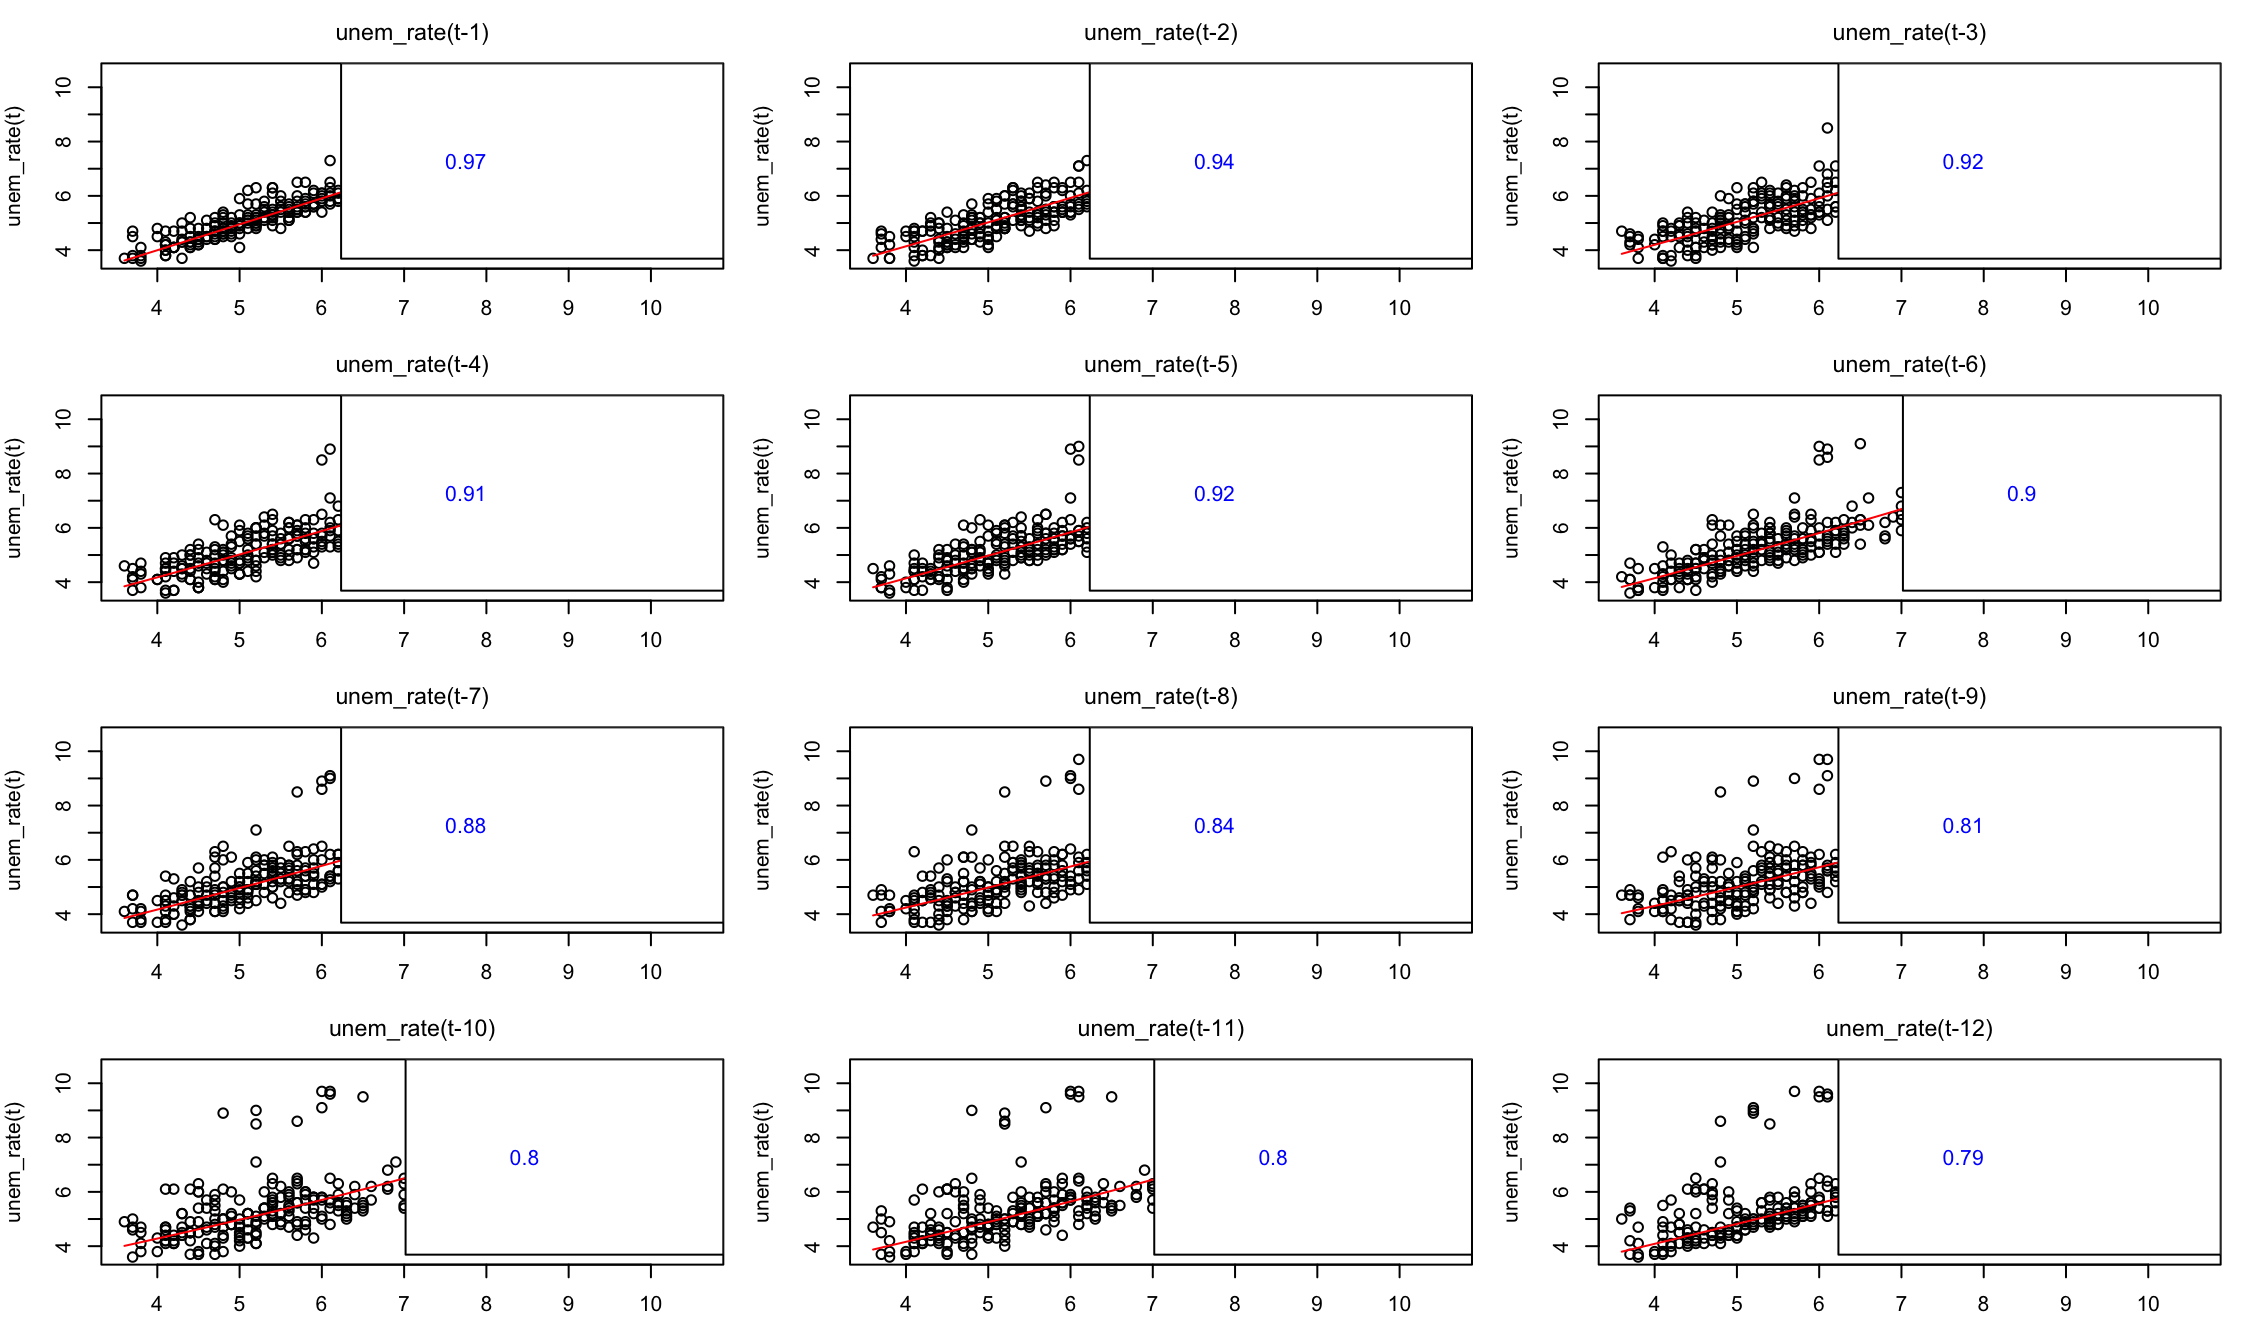
\includegraphics[width=\linewidth]{images/laggedunemployment}
	\end{figure}
			


					\begin{figure}[H]
		\centering
		\caption{Timeplots with and without differencing}
		\label{fig:seasonalunem}
		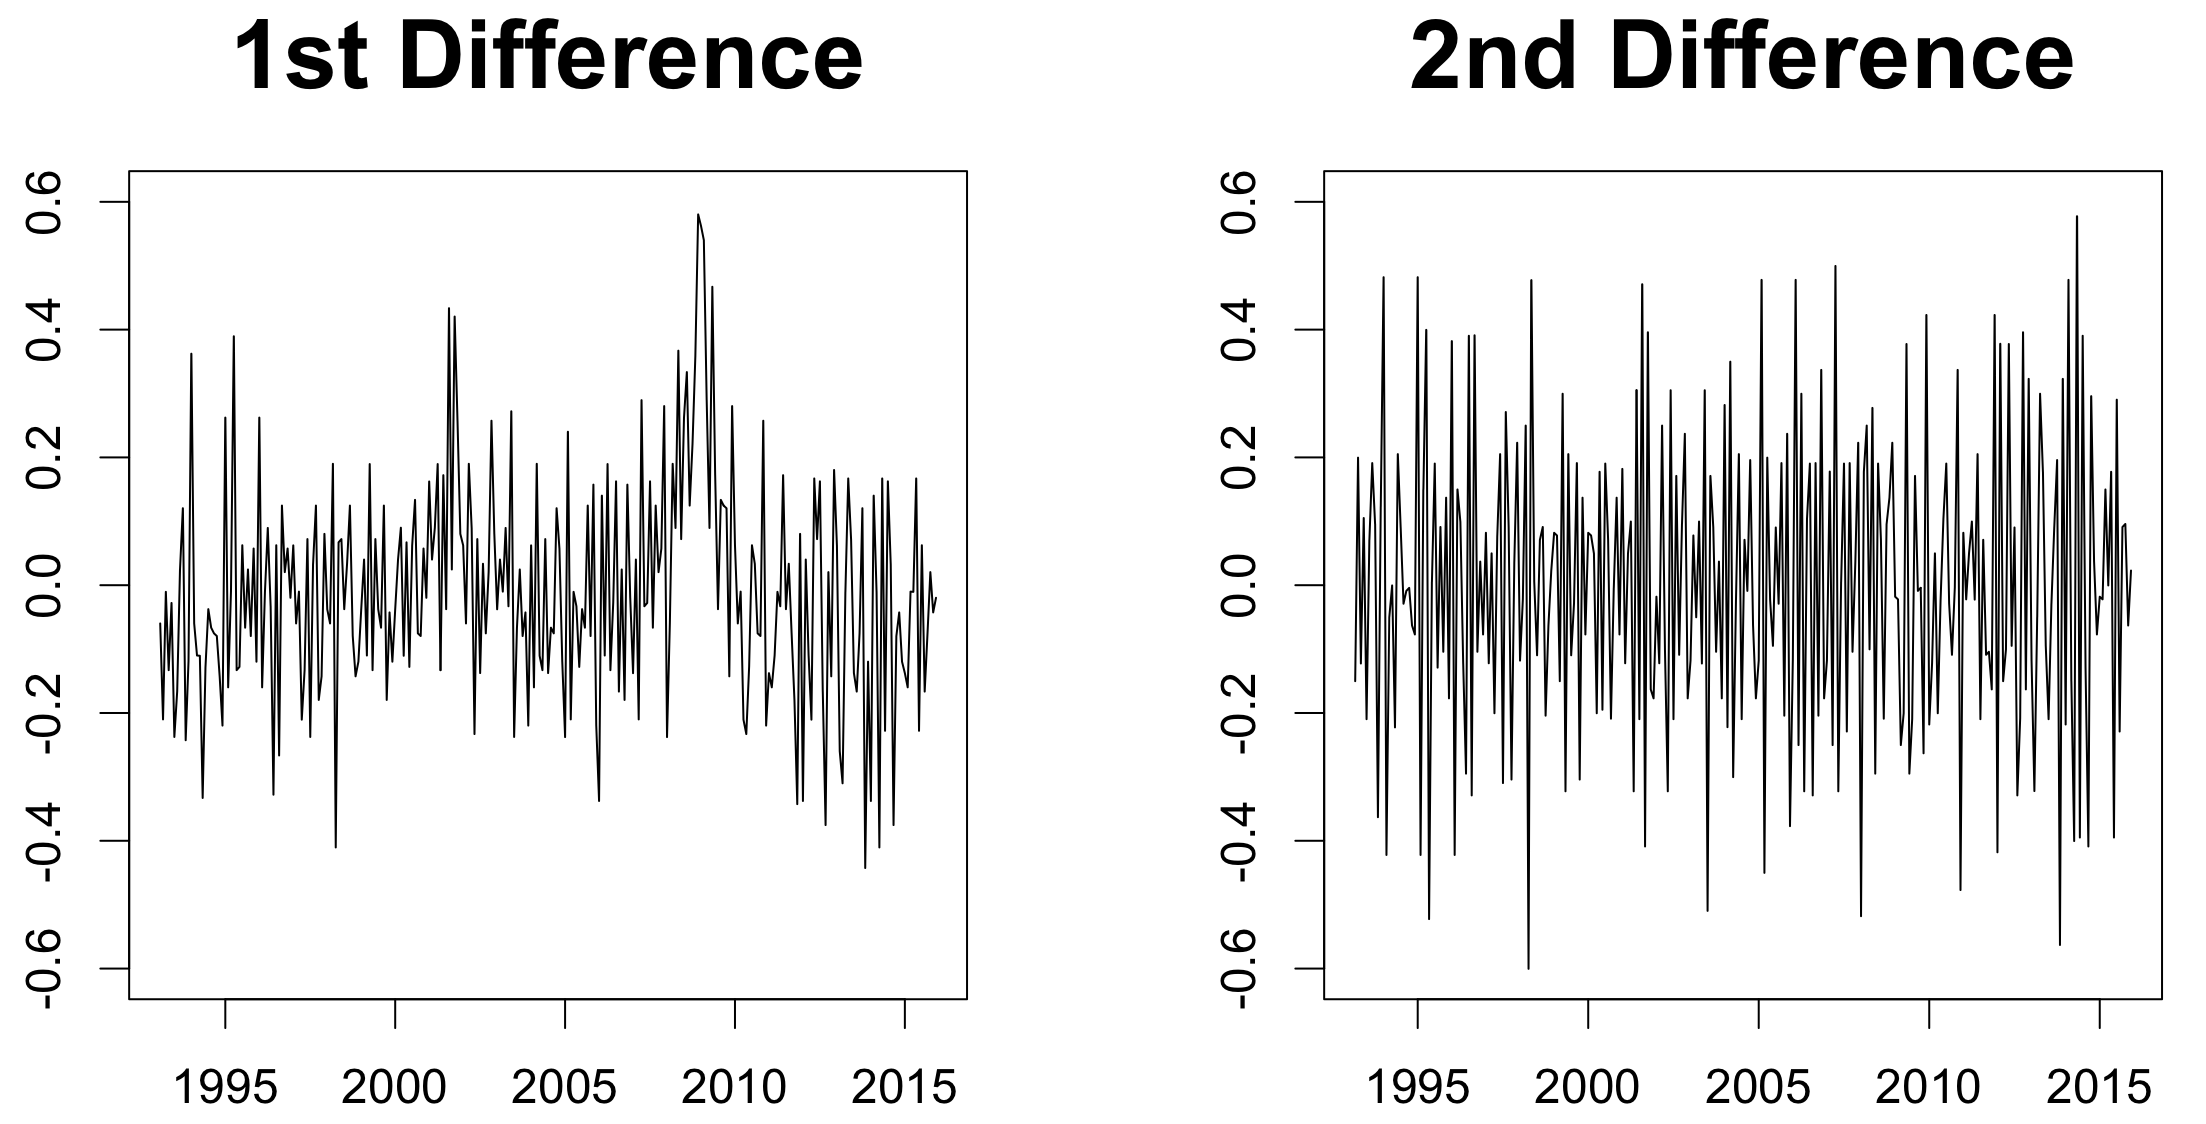
\includegraphics[width=\linewidth]{images/seasonalunem}
	\end{figure}

The first, second, and third differences of the unemployment data were plotted for seasonally adjusted unemployment data, see Figure \ref{fig:seasonalunem}. All three sets of differencing, bring the data closer to homoscedasticity. The  The associated ADF test results are given in Table \ref{tab:ADF}. Based on the p-values, there is significant evidence of stationarity with each of the differenced models. Visually the second differences best approximate a white noise series. Futhermore, even though the ADF statistic is more negative for the \(3^{rd}\) differences, in effort to build a parsimonious model  the consensus in the group was to continue the model building process using second differences.

	 \begin{table}[H]
		 \centering
		 \caption{ADF Test Results}
		 \label{tab:ADF}
		 \begin{tabular}{lllll}
		 \hline
		 \textbf{Model} & \textbf{Statistic} & \textbf{Lag order} & \textbf{p-value}\\ \hline
		  1\(^{st}\) difference &  -9.3595 & 6 &\( < 0.01\)\\
		  2\(^{nd}\) difference &  -9.3595 & 6 & \( < 0.01\)\\			  
		  3\(^{rd}\) difference &  -13.02 & 6 & \( < 0.01\)\\		 \hline
		 \end{tabular}
		 \end{table}

  


%------------------------------------------------

\section{Model Building}

\subsection{ACF and PACF Plots}
  
  \begin{figure}[H]
    	\centering
     	\caption{ACF \& PACF Plots}
     	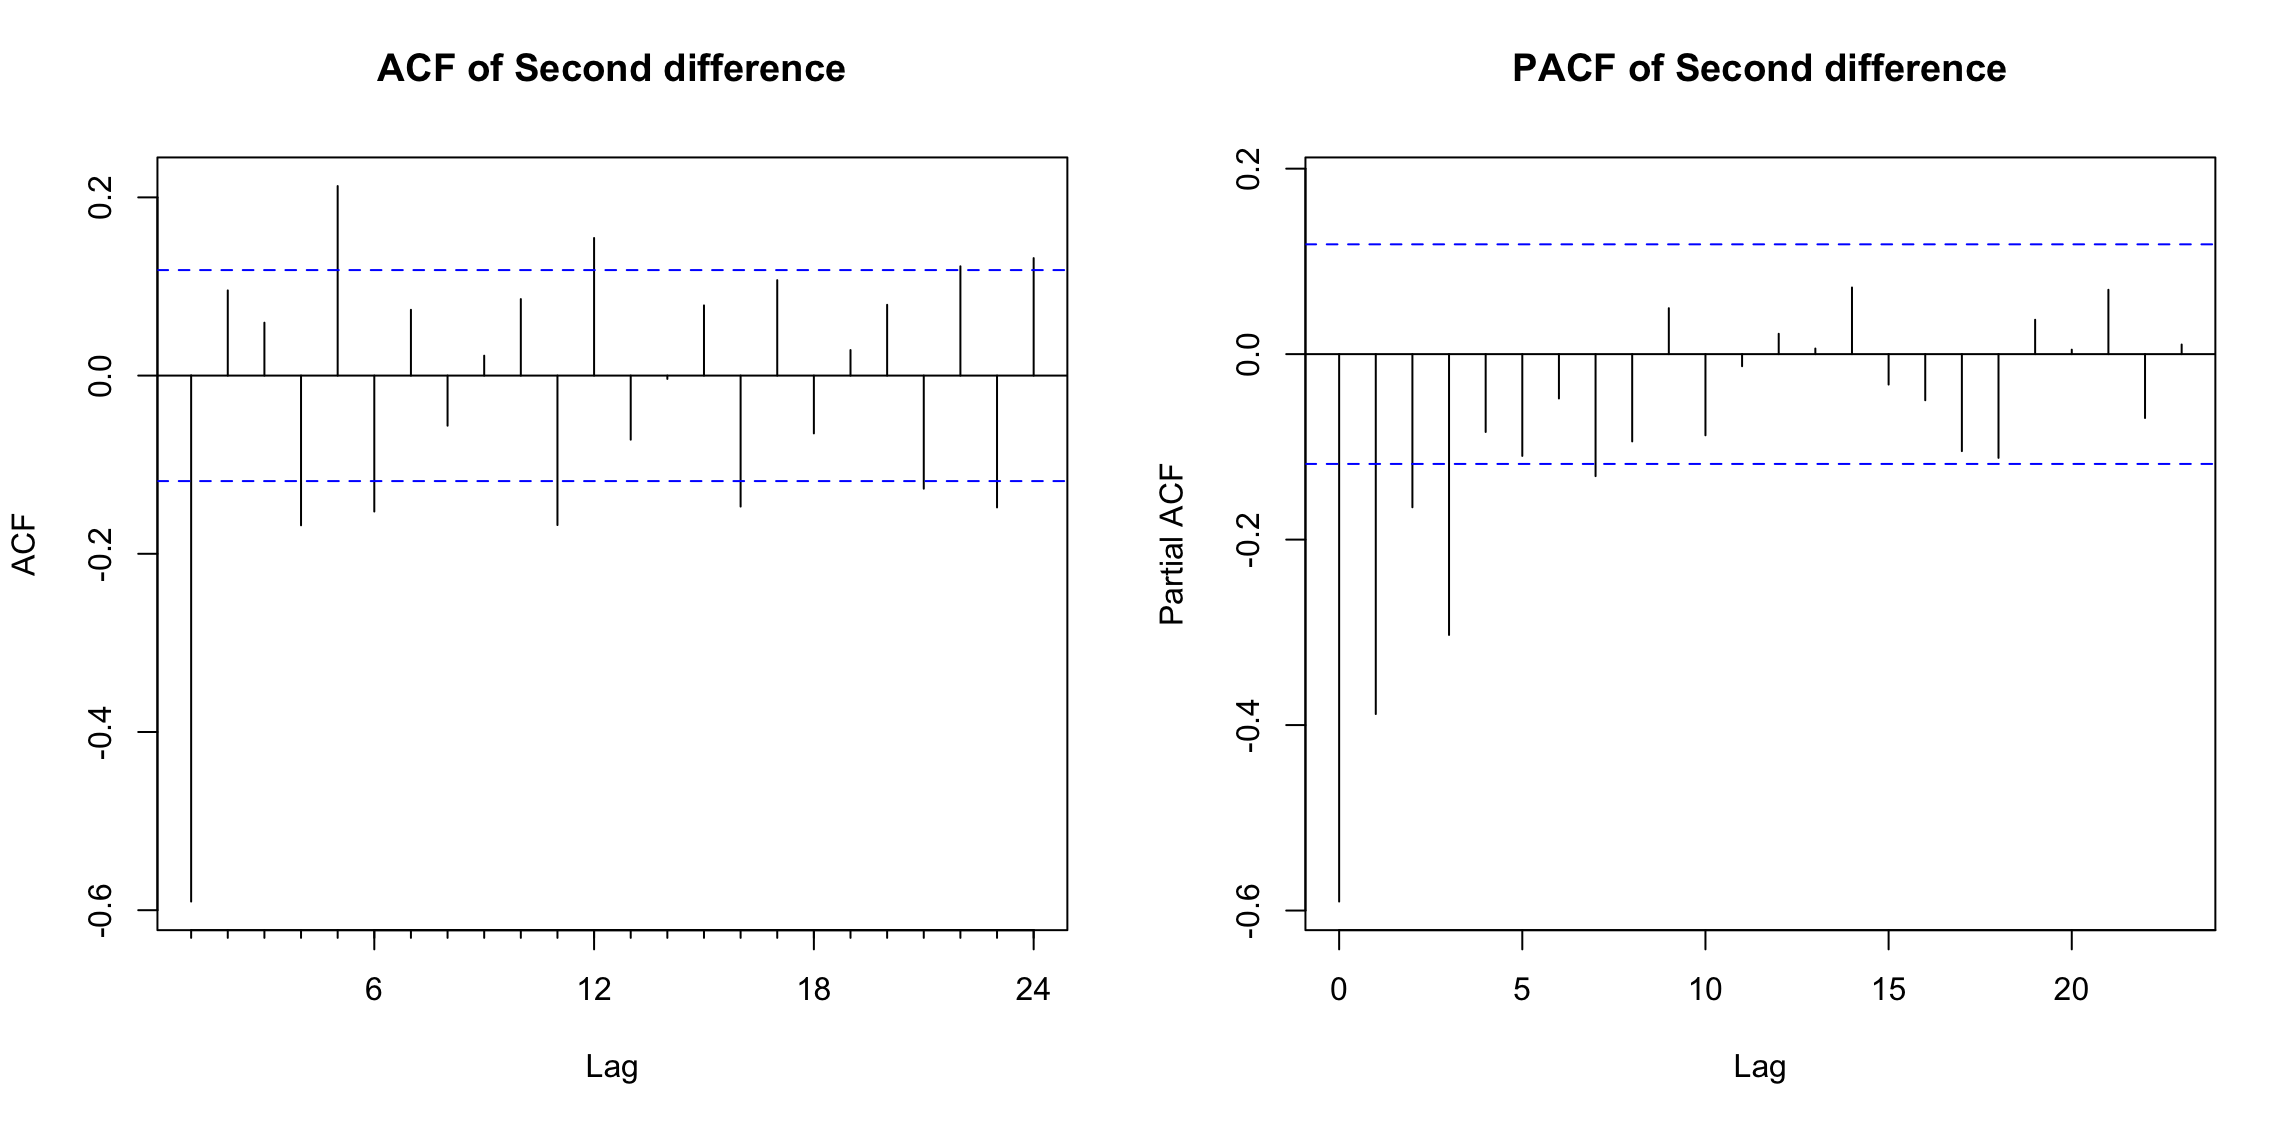
\includegraphics[width=\linewidth]{images/acfpacf}
     	\label{fig:secdiff2}
      \end{figure}
      
      The team visually analyzed the ACF and PACF plots within the first season (h = 1, 2, ..., 12), see Figure \ref{fig:secdiff2}. The PACF appears to decline slowly, while the ACF seems to fall off after 1. Therefore we began by letting p = 0, and q = 1. Several models were considered by making adjustments to variations resulting in the models found in Table \ref{tab:models}.\newline
      
      \subsection{Model Fit}
      
% latex table generated in R 3.3.1 by xtable 1.8-2 package
% Sun Jul 24 08:35:48 2016
\begin{table}[ht]
\centering
\begin{tabular}{cllrrl}
  \hline
 Model & Order & Reg  & AIC & BIC & Best \\ 
  \hline
1 & 1,2,1 &  NA &   -212.30 & -201.46 & BIC \\ 
  2  & 2,2,2 & NA   & -211.81 & -193.74 &  \\ 
  3  & 3,2,3 &  NA  & -215.48 & -190.19 &  \\ 
  4  & 1,2,1 & X  & -211.56 & -182.65 &  \\ 
  5  & 2,2,2 & X   & -209.83 & -177.32 &  \\ 
  6  & 3,2,3 & X   & -215.10 & -171.74 &  \\ 
  7  & 1,2,1 &  LagX & -222.45 & -193.69 & AIC \\ 
  8  & 2,2,2 &  LagX & -220.70 & -188.35 &  \\ 
  9  & 3,2,3 &  LagX & -217.89 & -174.76 &  \\ 
   \hline
\end{tabular}
\end{table}

% latex table generated in R 3.3.1 by xtable 1.8-2 package
% Sun Jul 24 08:35:48 2016
\begin{table}[ht]
\centering
\begin{tabular}{clllll}
  \hline
 Model & P & Type &  AIC & BIC & Best \\ 
  \hline
1  & 1 & NA  &  -223.67 & -201.97 &  \\ 
  2  & 2 & NA  &   -217.83 & -185.31 &  \\ 
  3  & 1 & Ind  & -256.77 & -231.45 & BIC/AIC \\ 
  4  & 1 & LagX & -216.65 & -195.06 &  \\ 
  5  & 2 & LagX & -212.53 & -180.17 &  \\ 
  6  & 1 & Both  & -245.72 & -220.53 &  \\ 
   \hline
\end{tabular}
\end{table}

% latex table generated in R 3.3.1 by xtable 1.8-2 package
% Sun Jul 24 08:35:48 2016
\begin{table}[ht]
\centering
\begin{tabular}{lllll}
  \hline
Model & Type & AIC & BIC & Best \\ 
  \hline
ARIMA(1,2,1) & NA &   -212.29 & -201.45 &  \\ 
ARIMA(1,2,1) & LagX   & -222.45 & -193.69 &  \\ 
VAR(1) & Ind & -256.76 & -231.45 & AIC/BIC \\ 
   \hline
\end{tabular}
\end{table}

		%-----------------------------------------------------------------------------------------
		
	\textbf{\textit{A lot of the commentary below is wrong now.  I am in the process of moving the information from what I gathered from our online discussions to here.}}
	
		Based on the AIC values, the two models that show the most promise are models 5 and 7.  Model 5 includes only the time series data whereas model 7 also includes some of the predictors of interest.  The diagnostic plots are shown in Figures \ref{fig:mod5} and \ref{fig:mod7}. Both models show a great deal of promise.  The standardized residuals show no apparent pattern. The ACF of the residuals show no departure from normality. Although the Normal Q-Q plot of the standardized residuals shows some slight departure from normality in the tails, there is no strong evidence of lack of normality in the residuals  The p-values for the  Ljung-Box statistic are high enough at all plotted lags, so there is no indication of lack of fit in the models. Therefore, we will continue to refine these models further as we explore the nature of US Unemployment rate patterns.


\subsection{Predictor Variables}

\blindtext % Dummy text

\section{Forcasting}

 \begin{figure}[H]
    	\centering
     	\caption{Forcasting with ARIMA and VAR models}
     	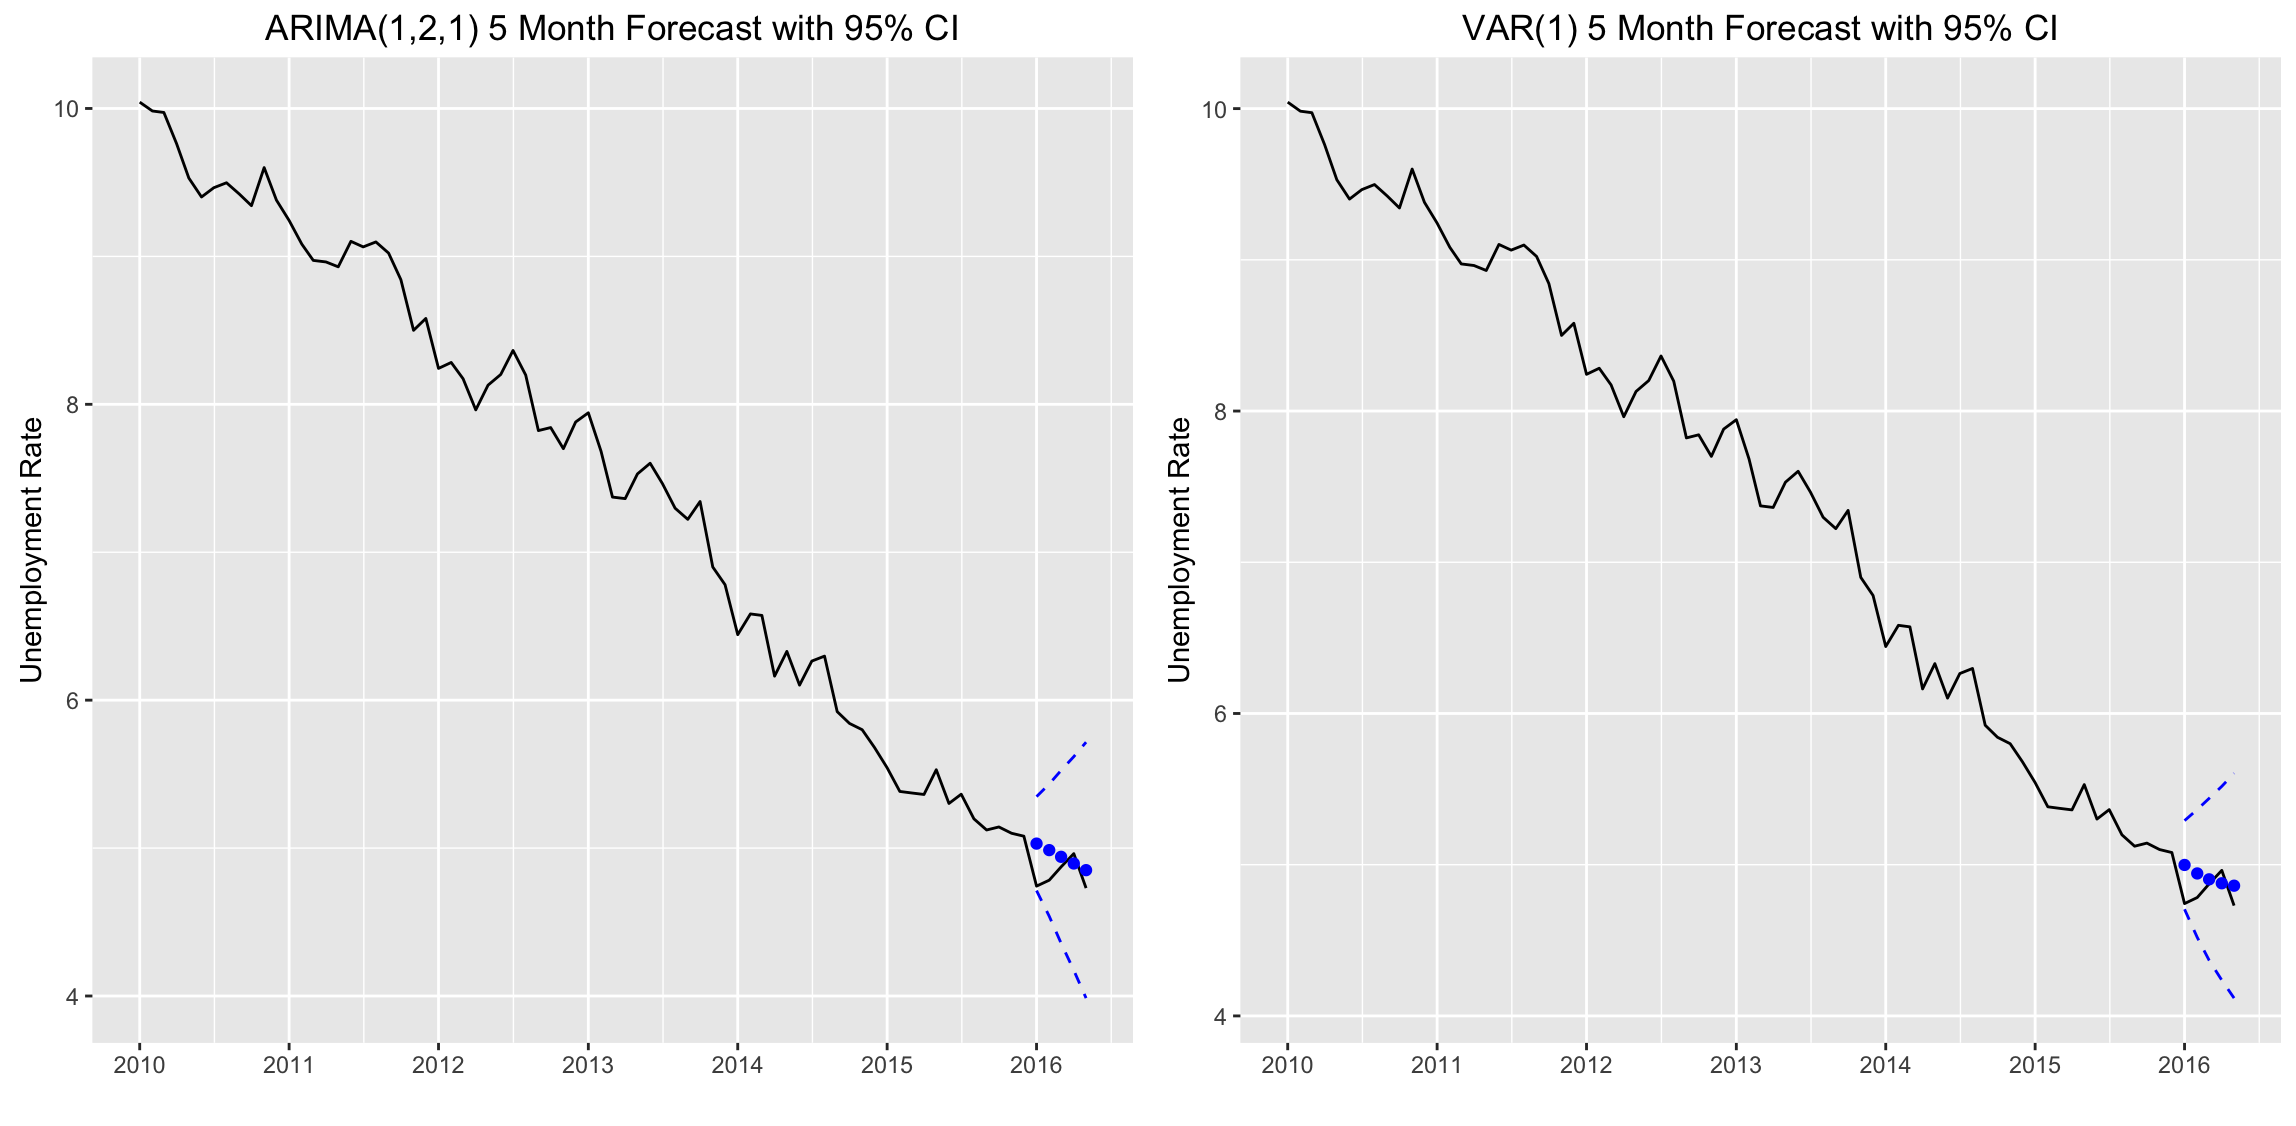
\includegraphics[width=\linewidth]{images/forcasts}
     	\label{fig:forcasts}
      \end{figure}
      
       \begin{figure}[H]
    	\centering
     	\caption{3 year forcasts}
     	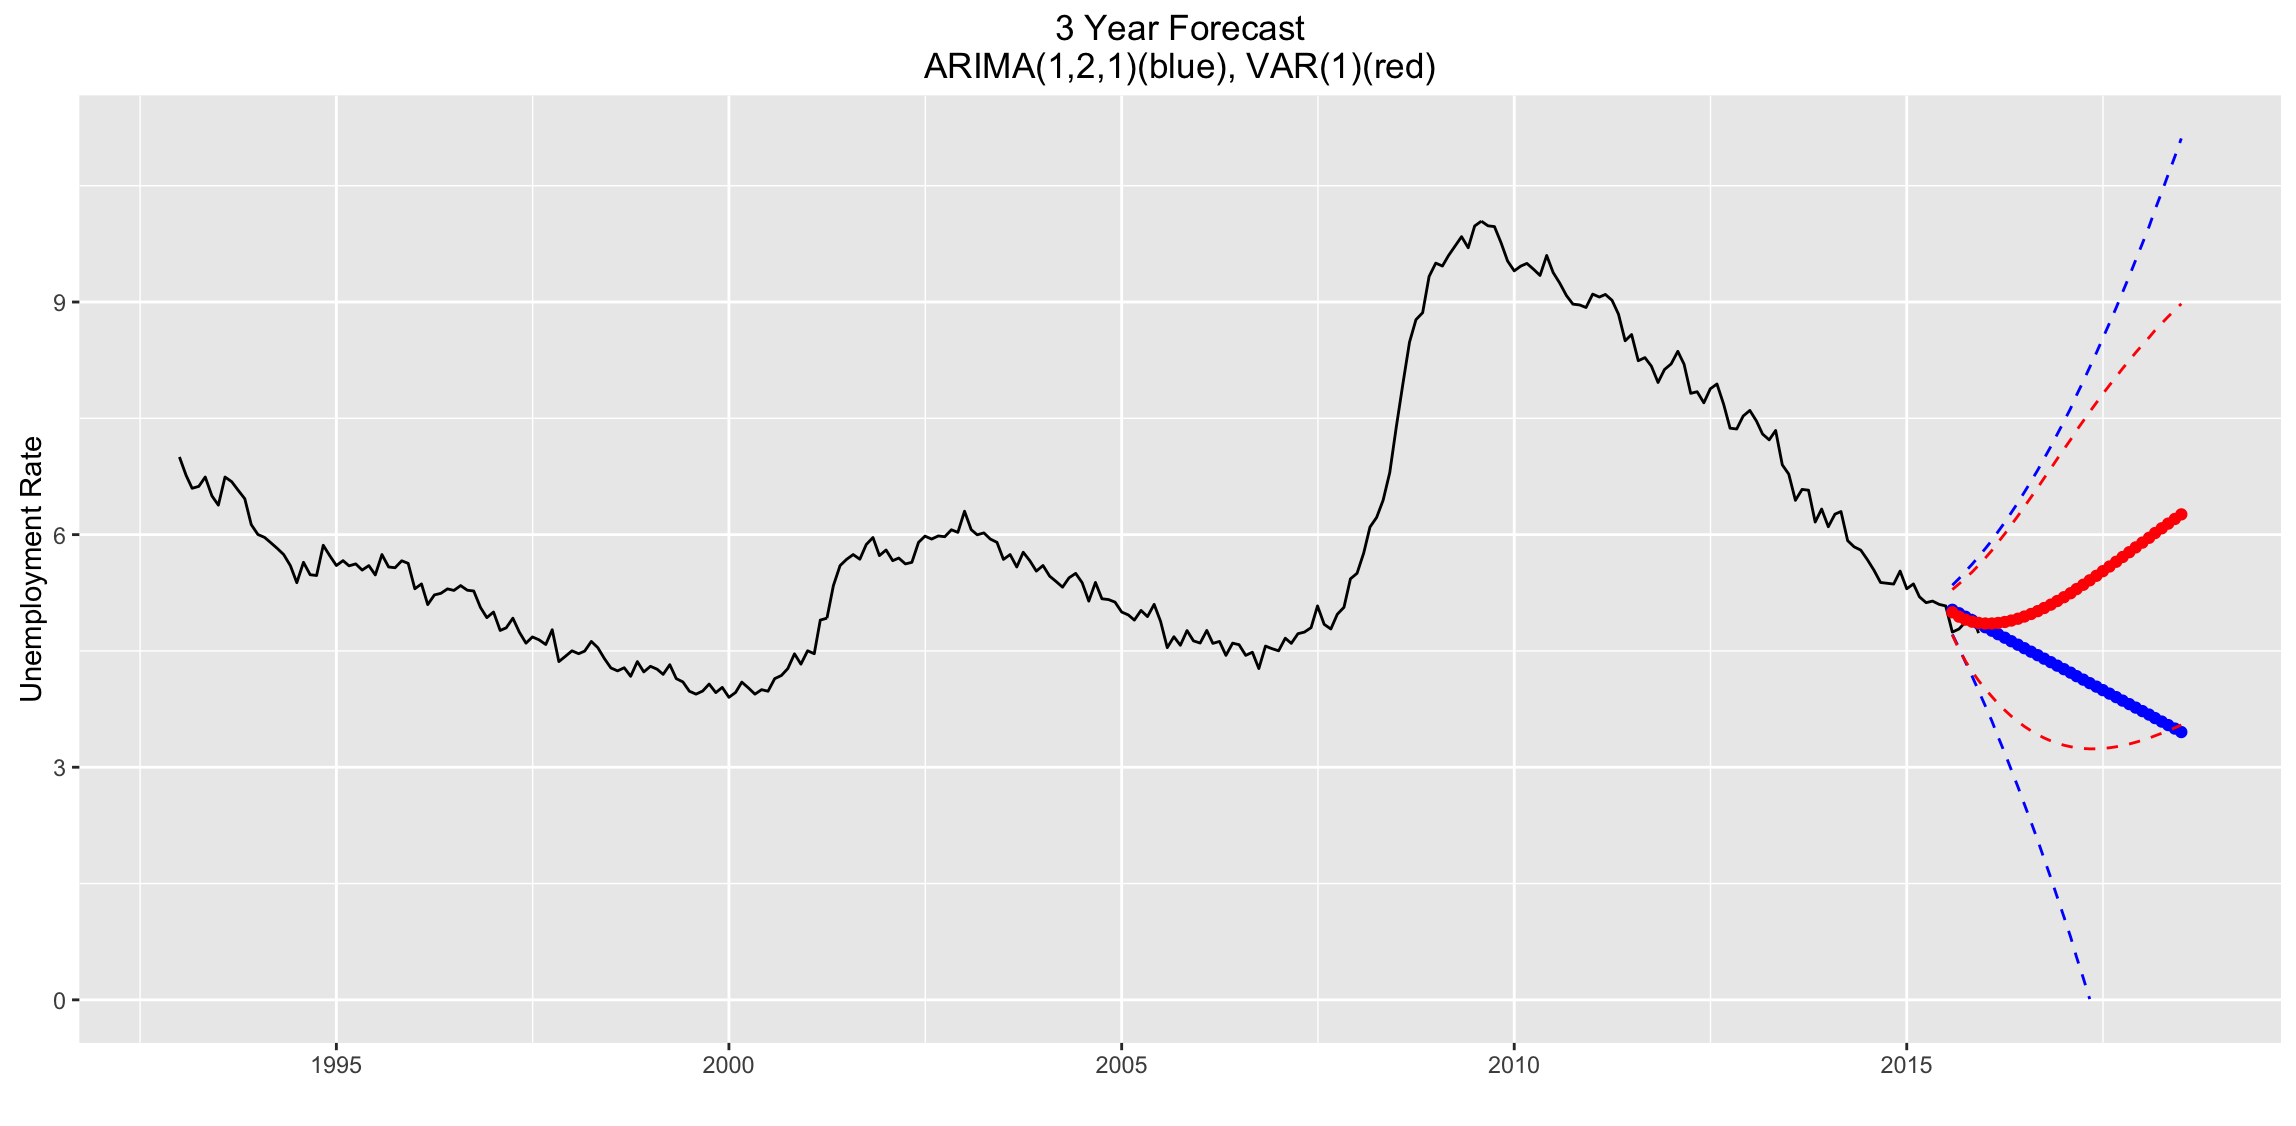
\includegraphics[width=\linewidth]{images/forcast3}
     	\label{fig:forcasts}
      \end{figure}

\section{Discussion and Implications}

\blindtext % Dummy text

%----------------------------------------------------------------------------------------
%	REFERENCE LIST
%----------------------------------------------------------------------------------------

\begin{flushleft}
\bibliography{main} % refers to our bibliography
\end{flushleft}

\appendix
\section{Appendix: Sarima output} \label{App:AppendixA}

       \begin{figure}[H]
    	\centering
     	\caption{Model 1}
     	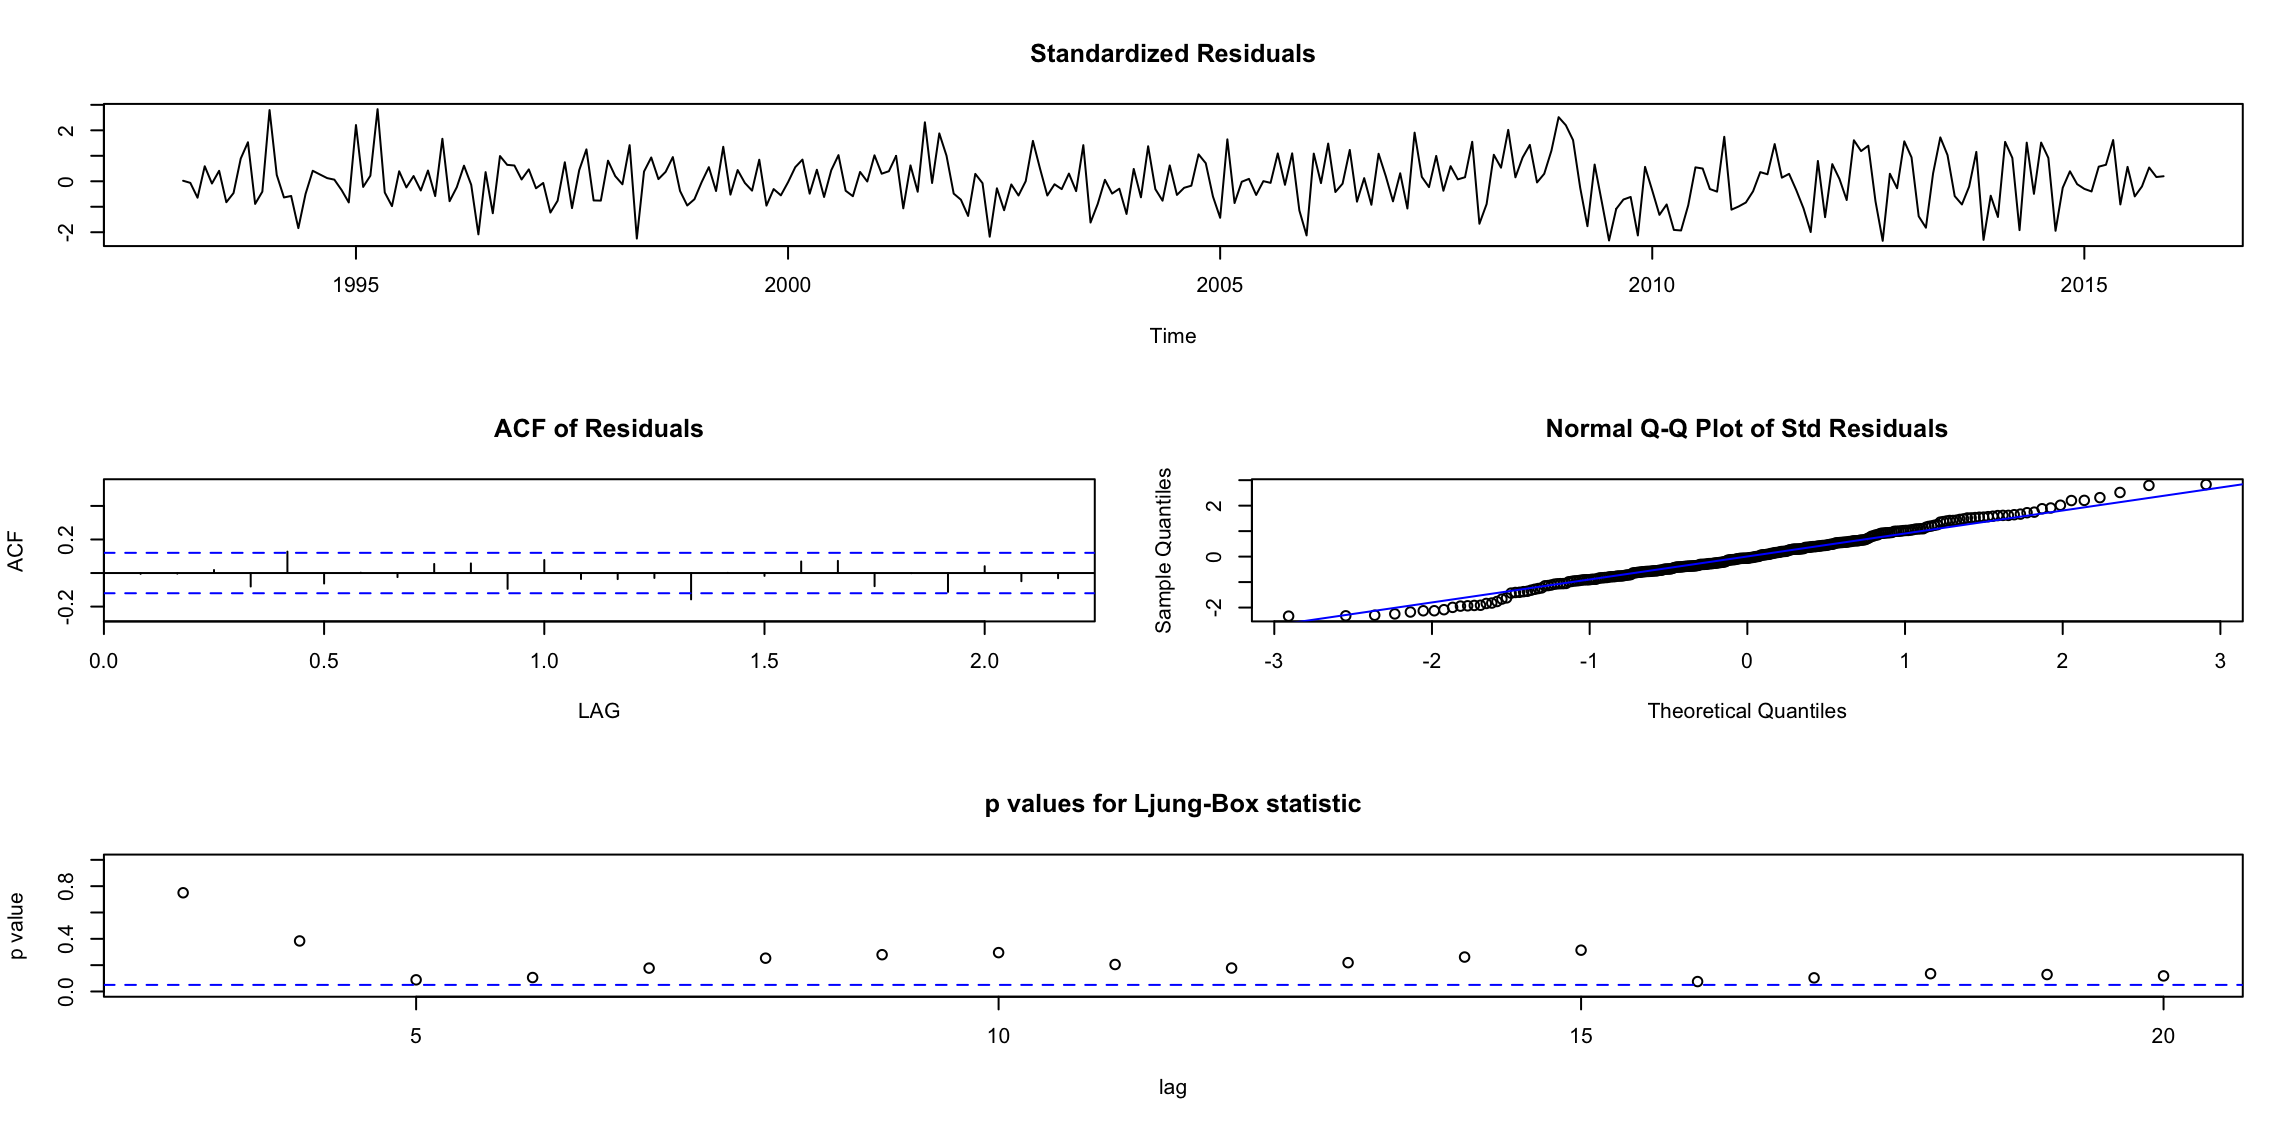
\includegraphics[width=\linewidth]{images/sarima1}
     	\label{fig:sarima1}
     	     	\caption{Model 2}
     	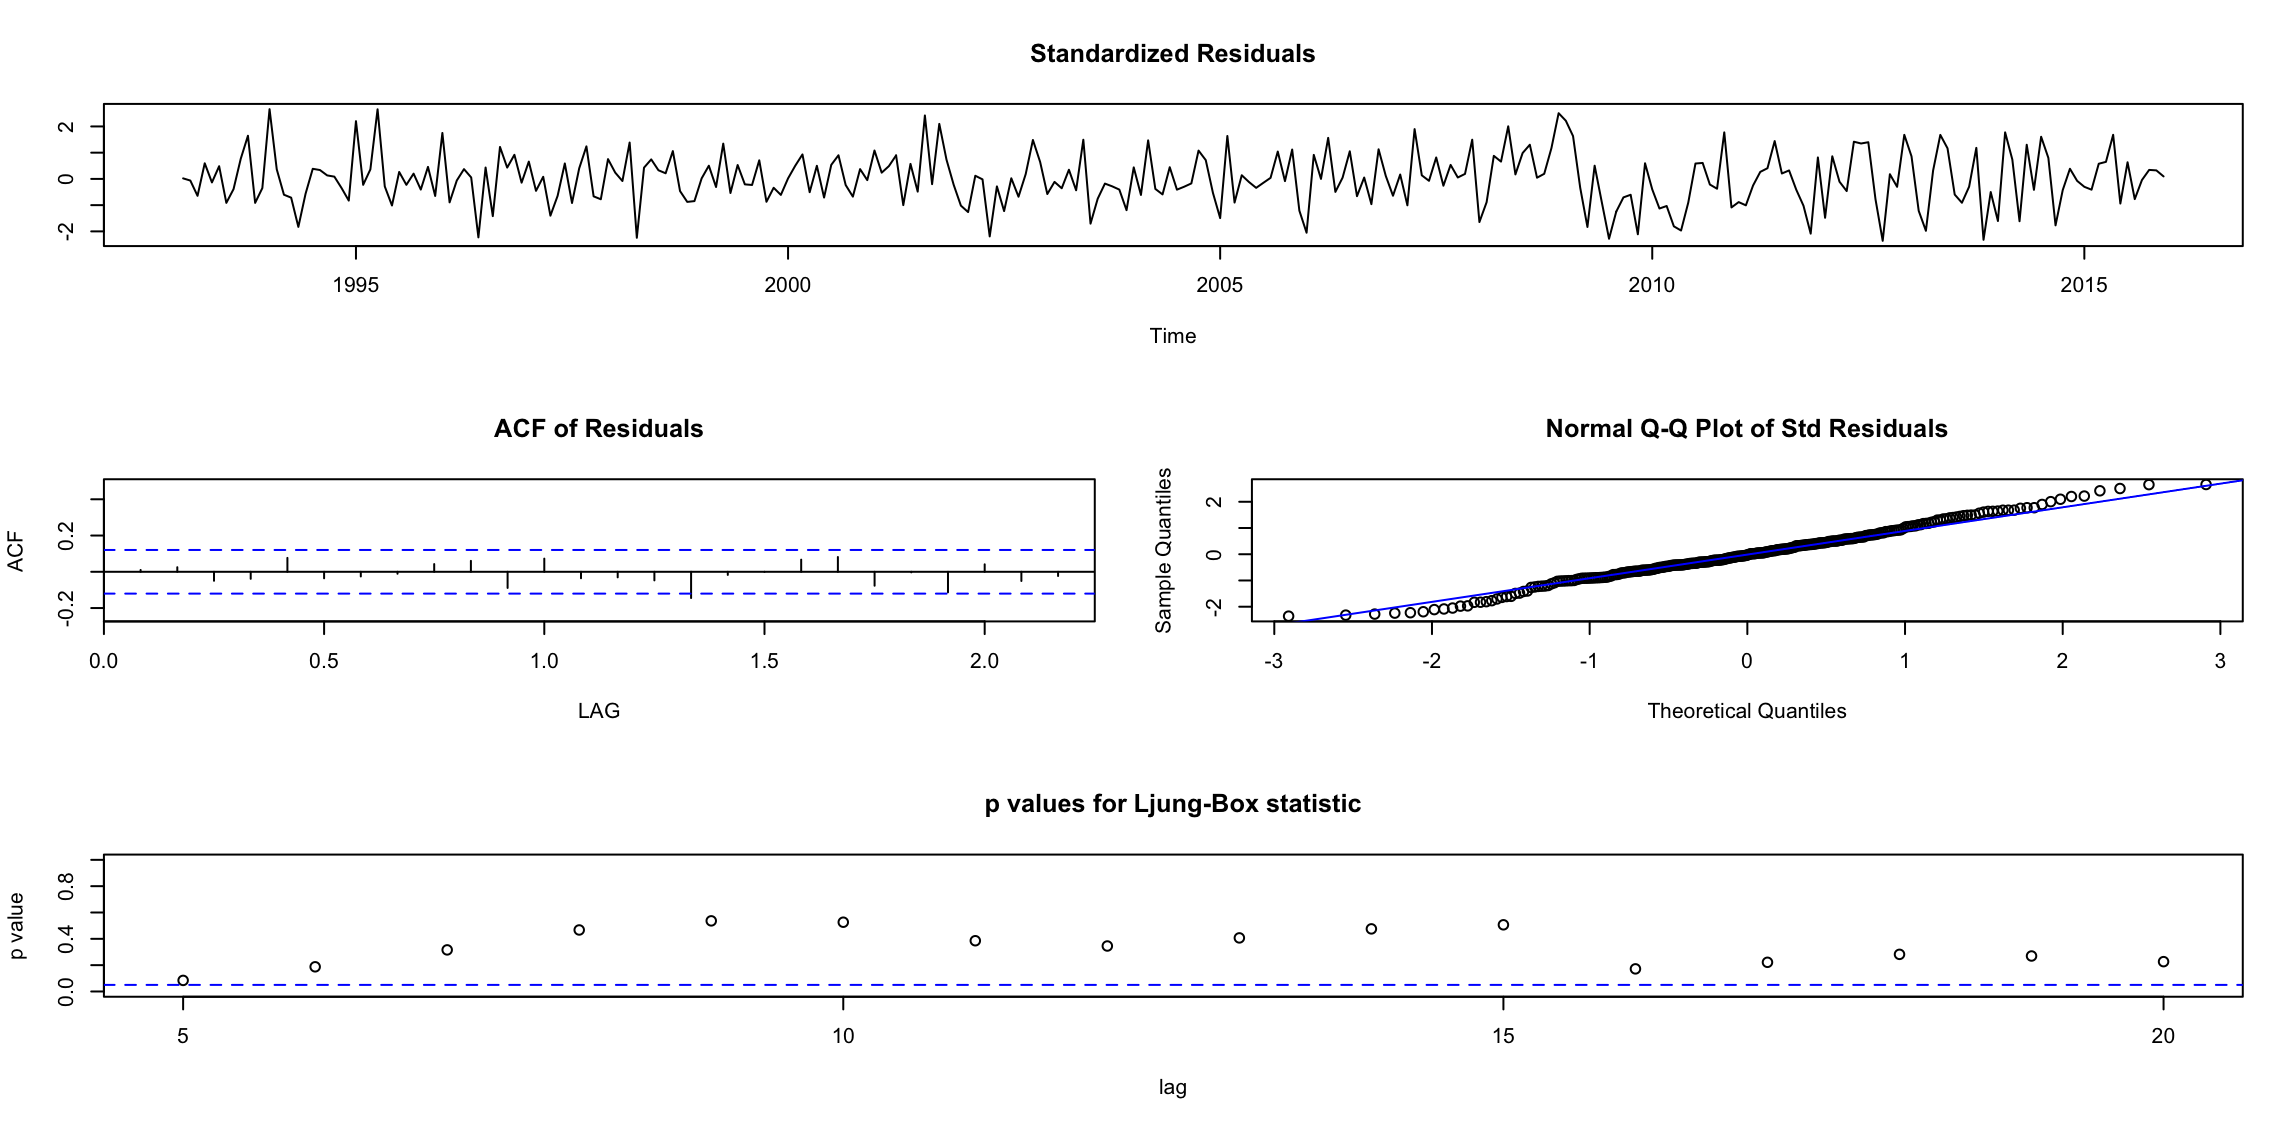
\includegraphics[width=\linewidth]{images/sarima2}
     	\label{fig:sarima2}
     	    	\caption{Model 3}
     	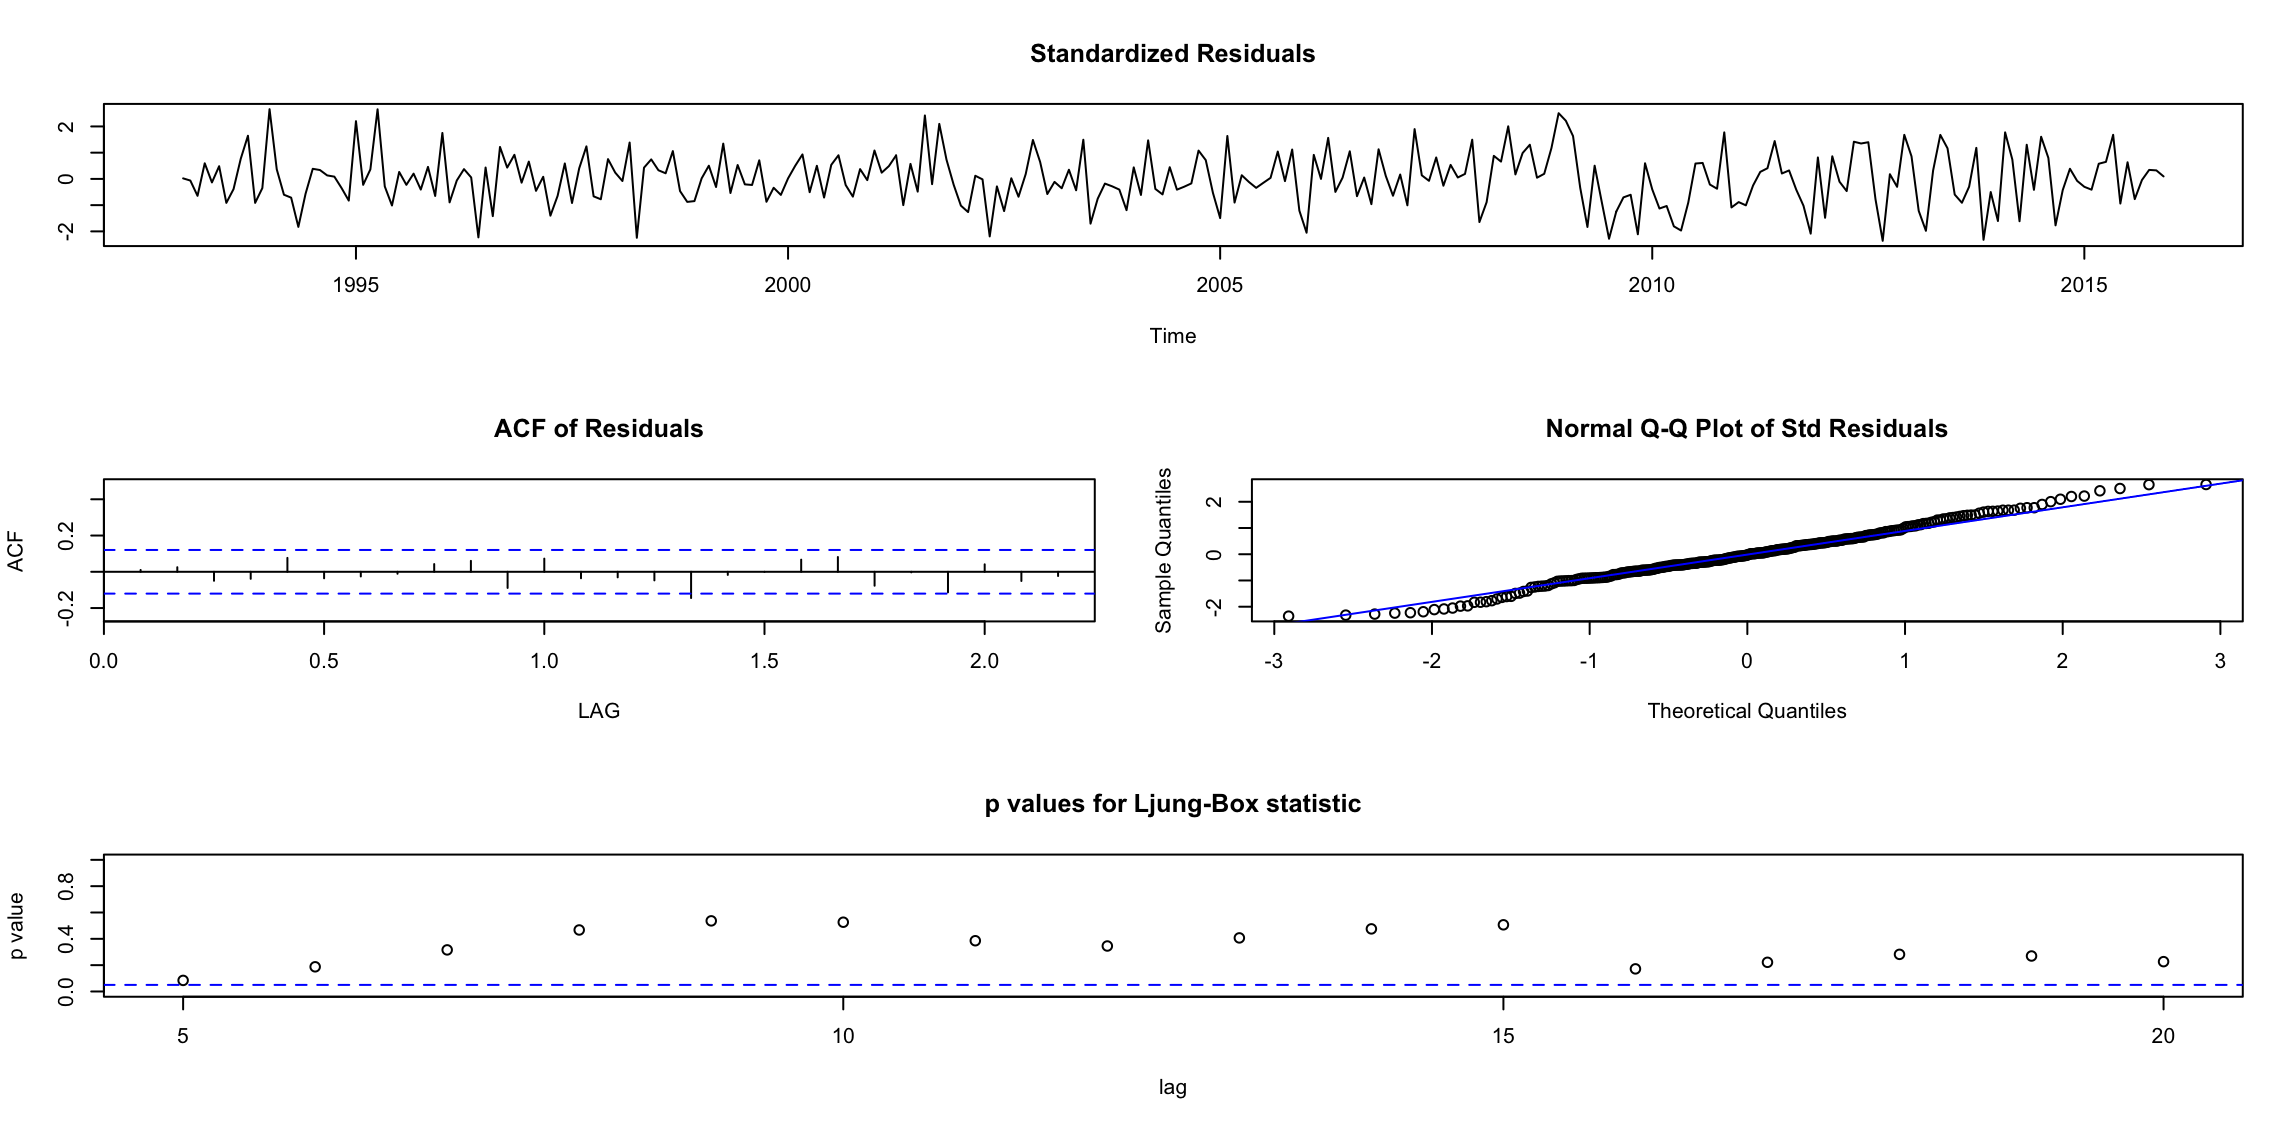
\includegraphics[width=\linewidth]{images/sarima3}
     	\label{fig:sarima3}
      \end{figure}
      
      
      
         \begin{figure}[H]
    	\centering
     	\caption{Model 4}
     	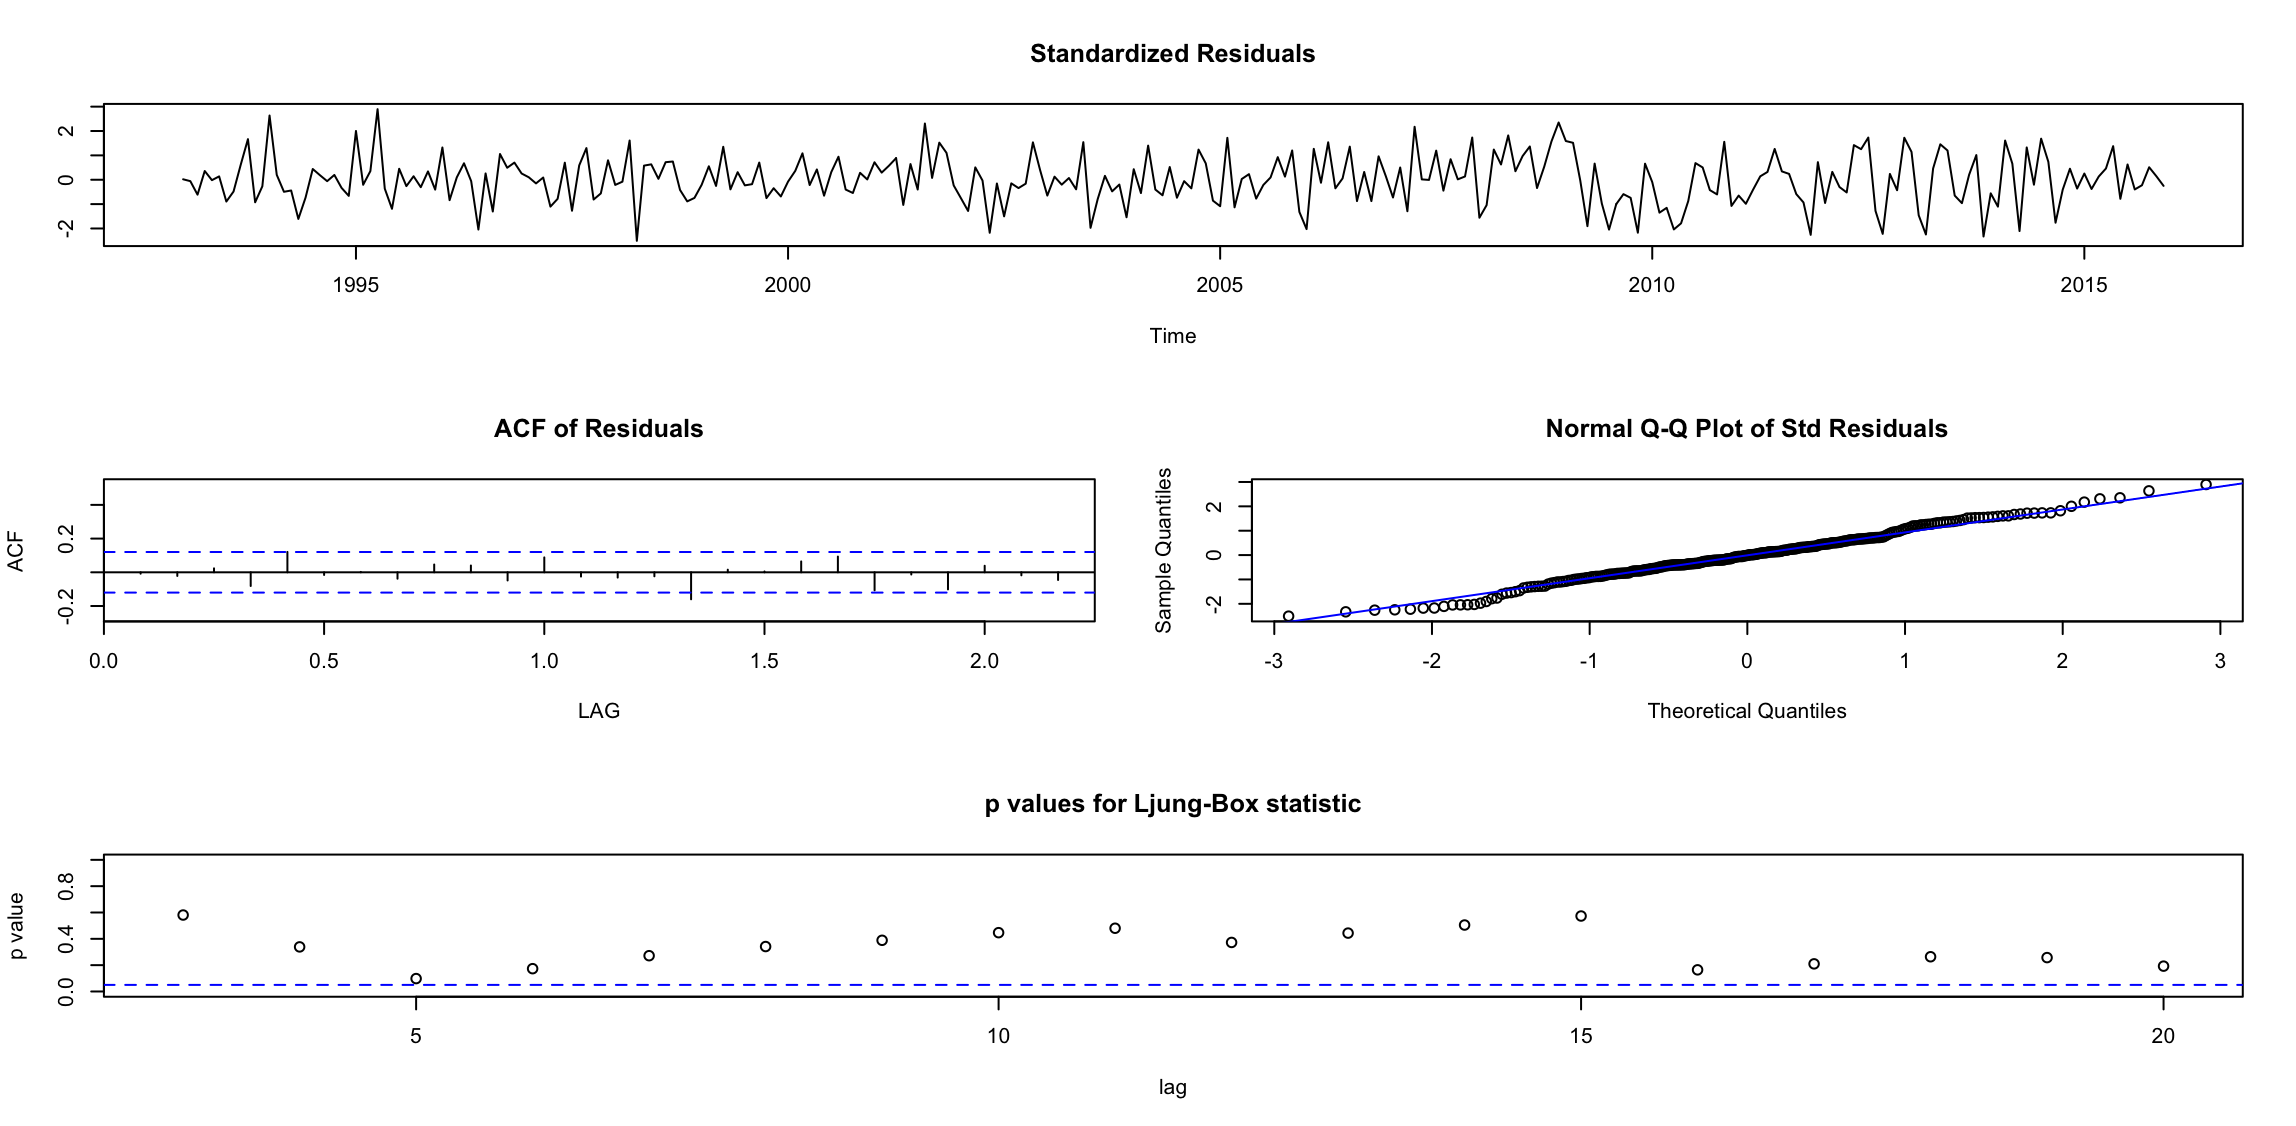
\includegraphics[width=\linewidth]{images/sarima4}
     	\label{fig:sarima4}
     	\caption{Model 5}
     	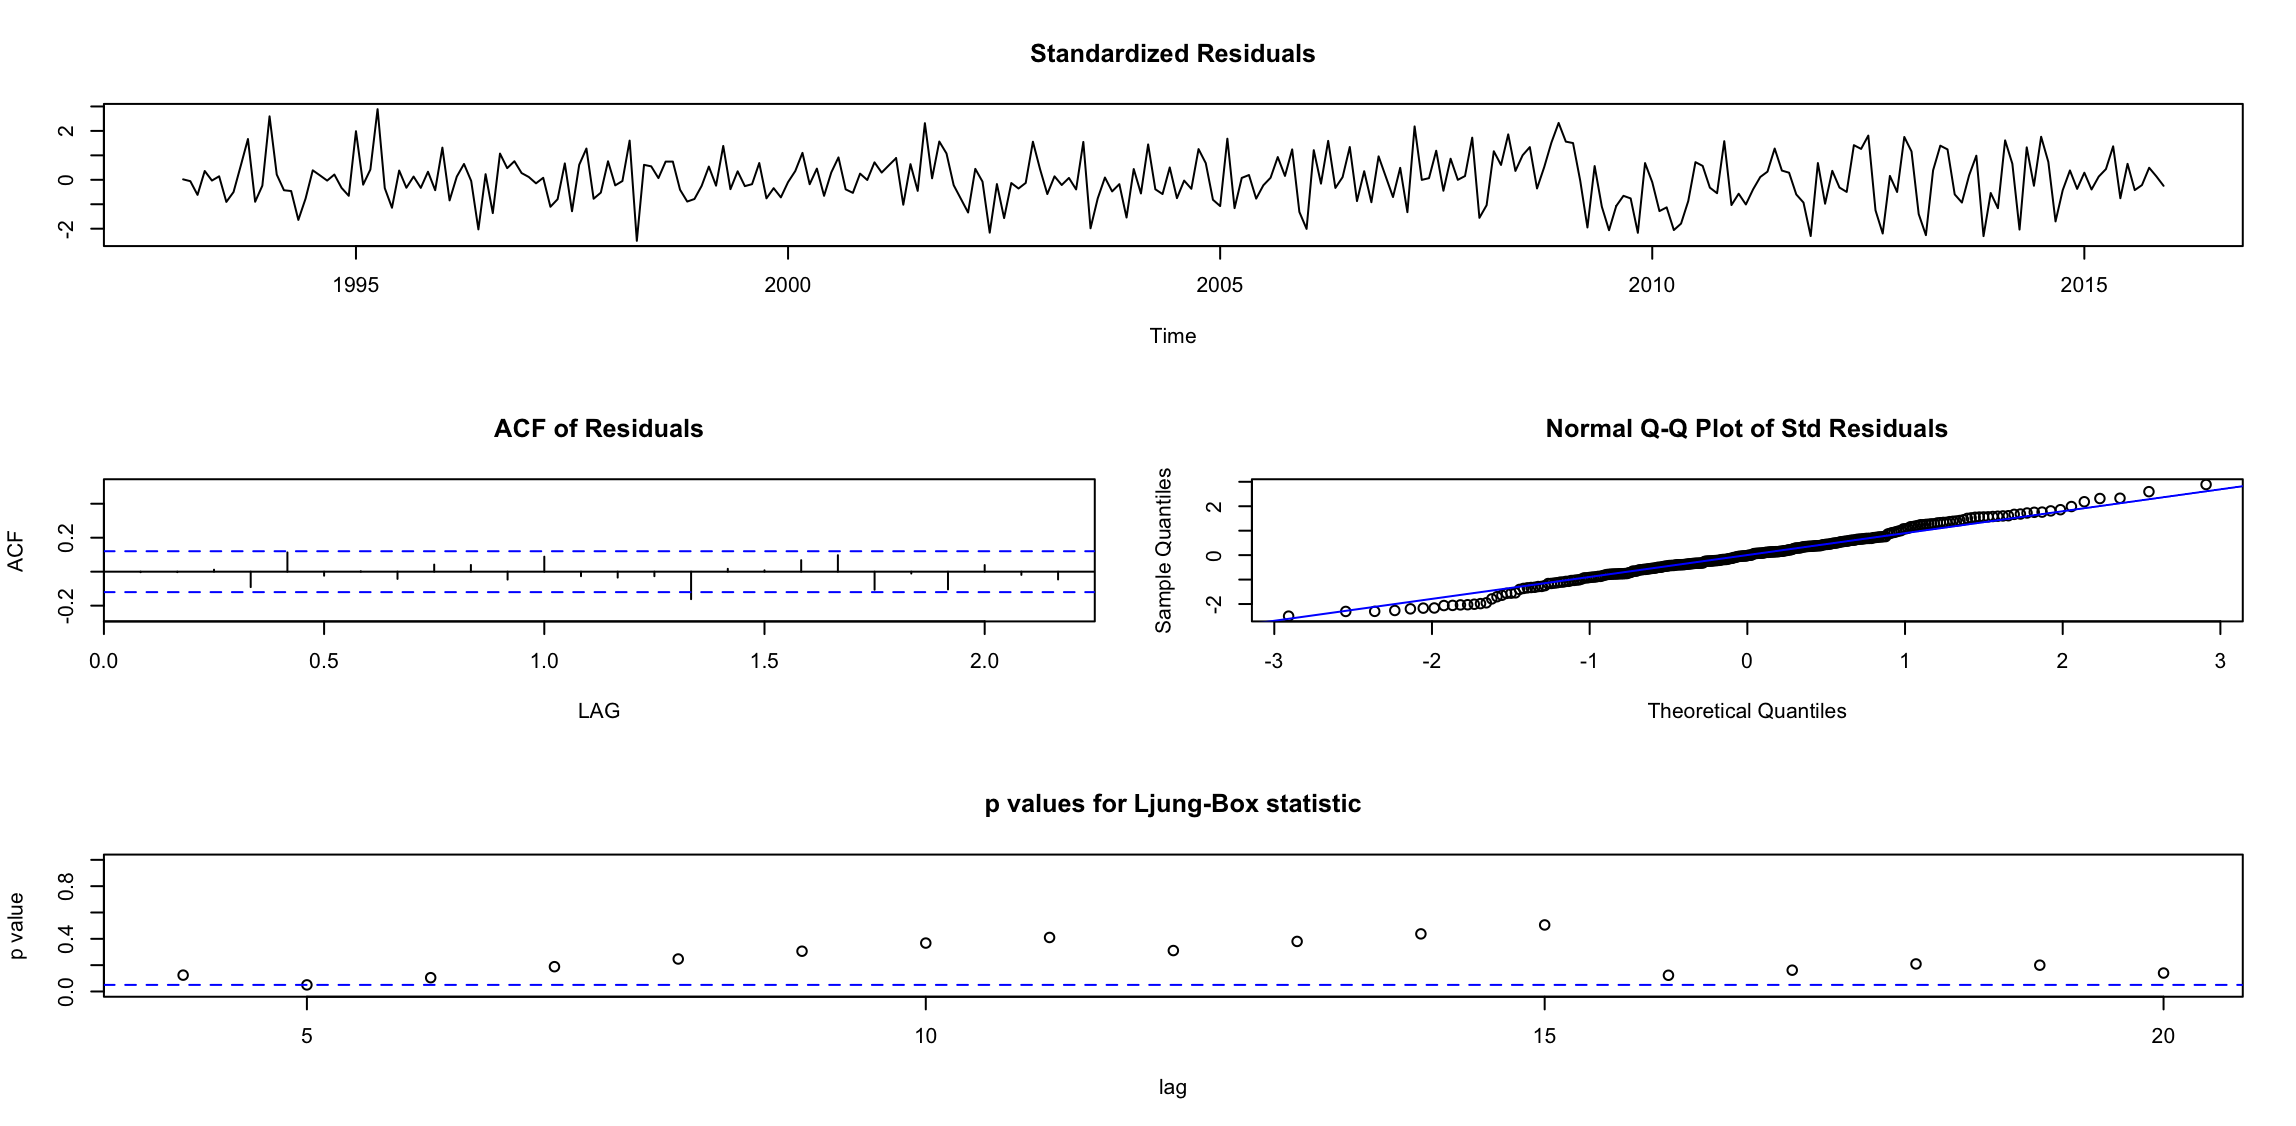
\includegraphics[width=\linewidth]{images/sarima5}
     	\label{fig:sarima5}
     	\caption{Model 6}
     	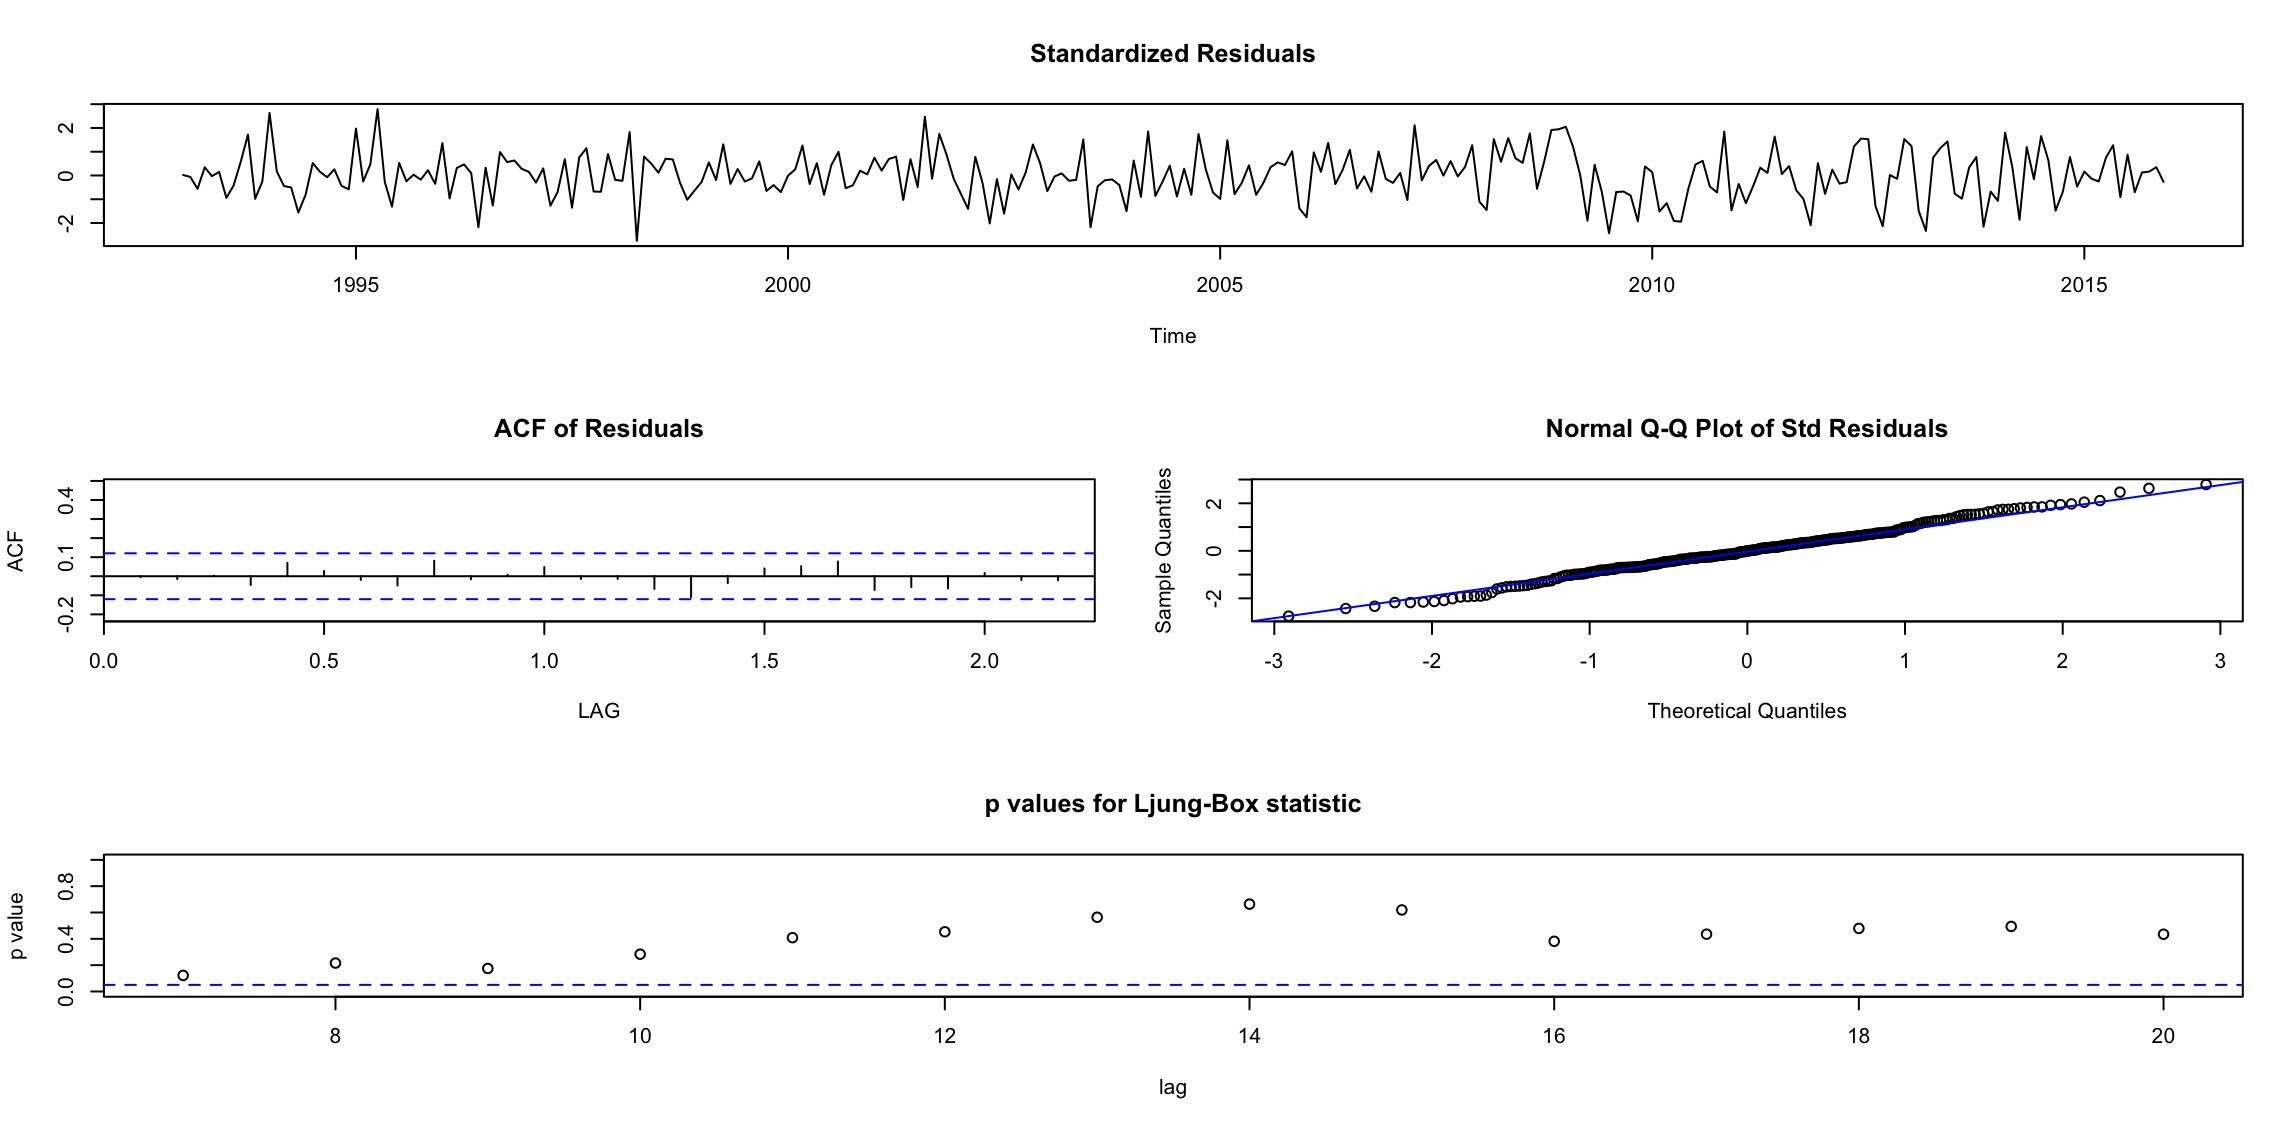
\includegraphics[width=\linewidth]{images/sarima6}
     	\label{fig:sarima6}
     	     	\caption{Model 7}
     	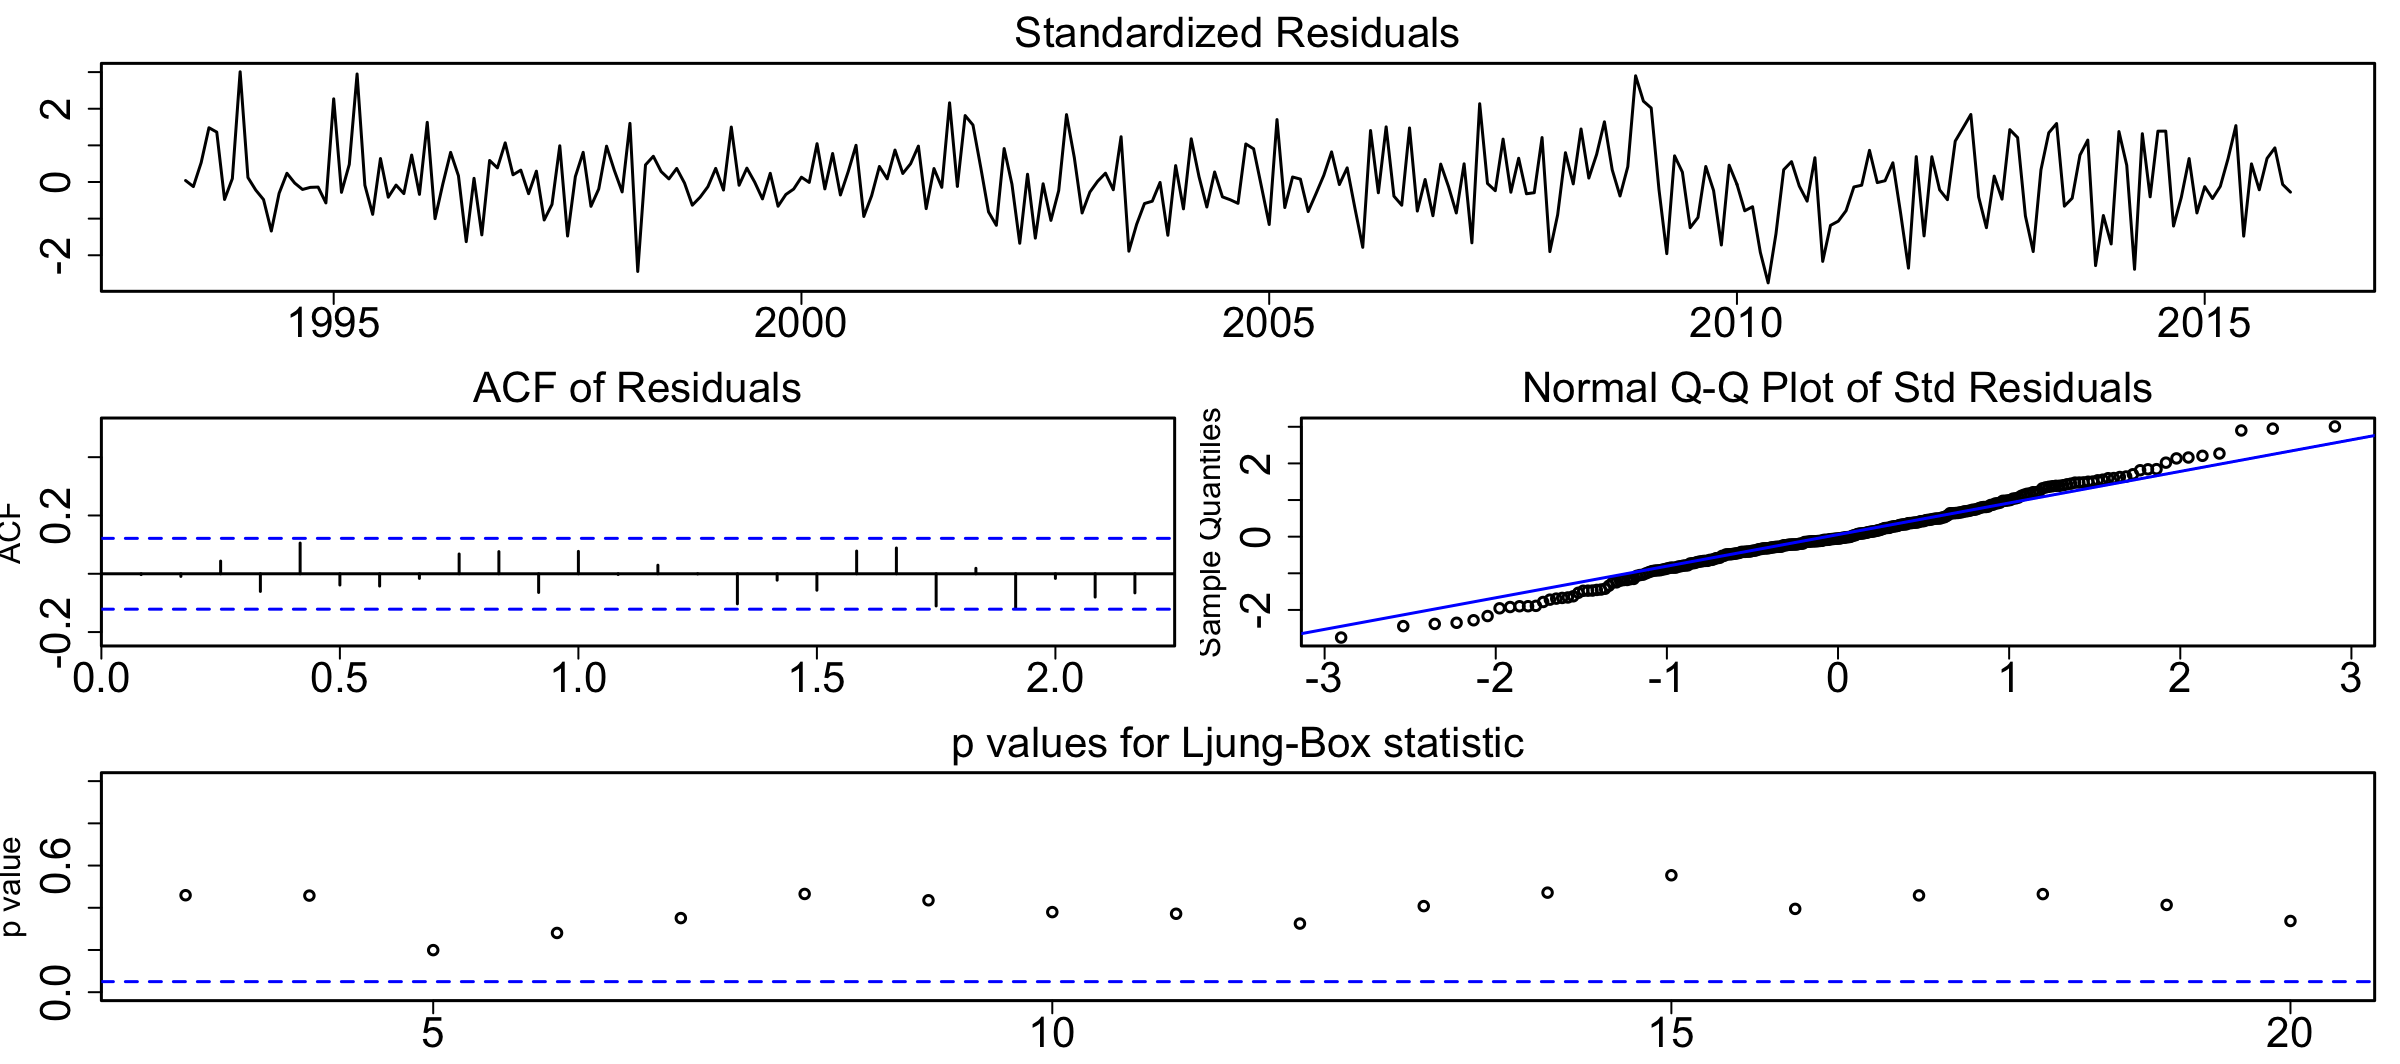
\includegraphics[width=\linewidth]{images/sarima7}
     	\label{fig:sarima7}
      \end{figure}

              \begin{figure}[H]
    	\centering
     	\caption{Model 8}
     	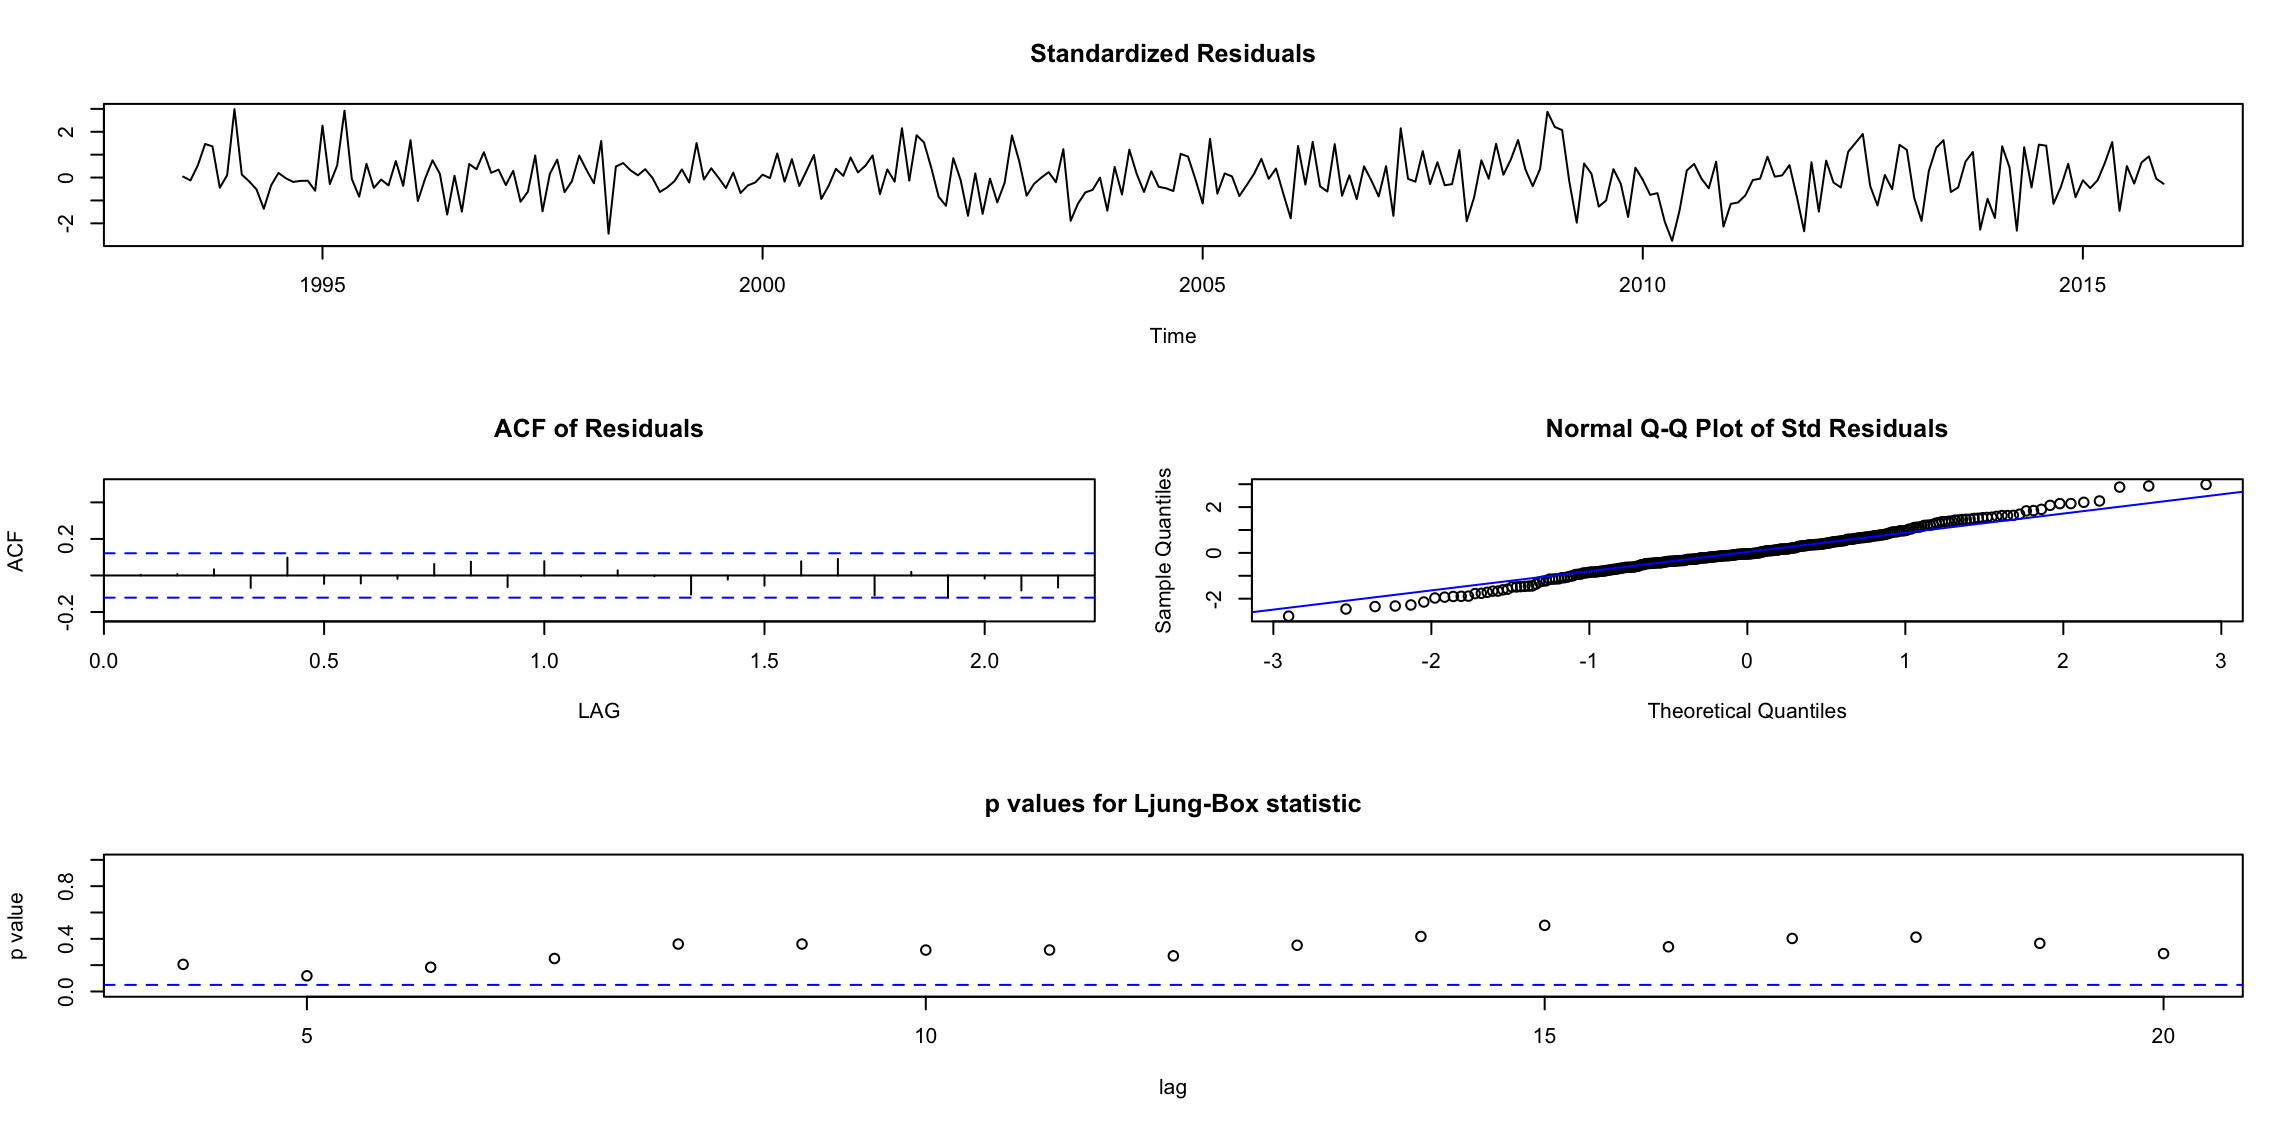
\includegraphics[width=\linewidth]{images/sarima8}
     	\label{fig:sarima8}
     	\caption{Model 9}
     	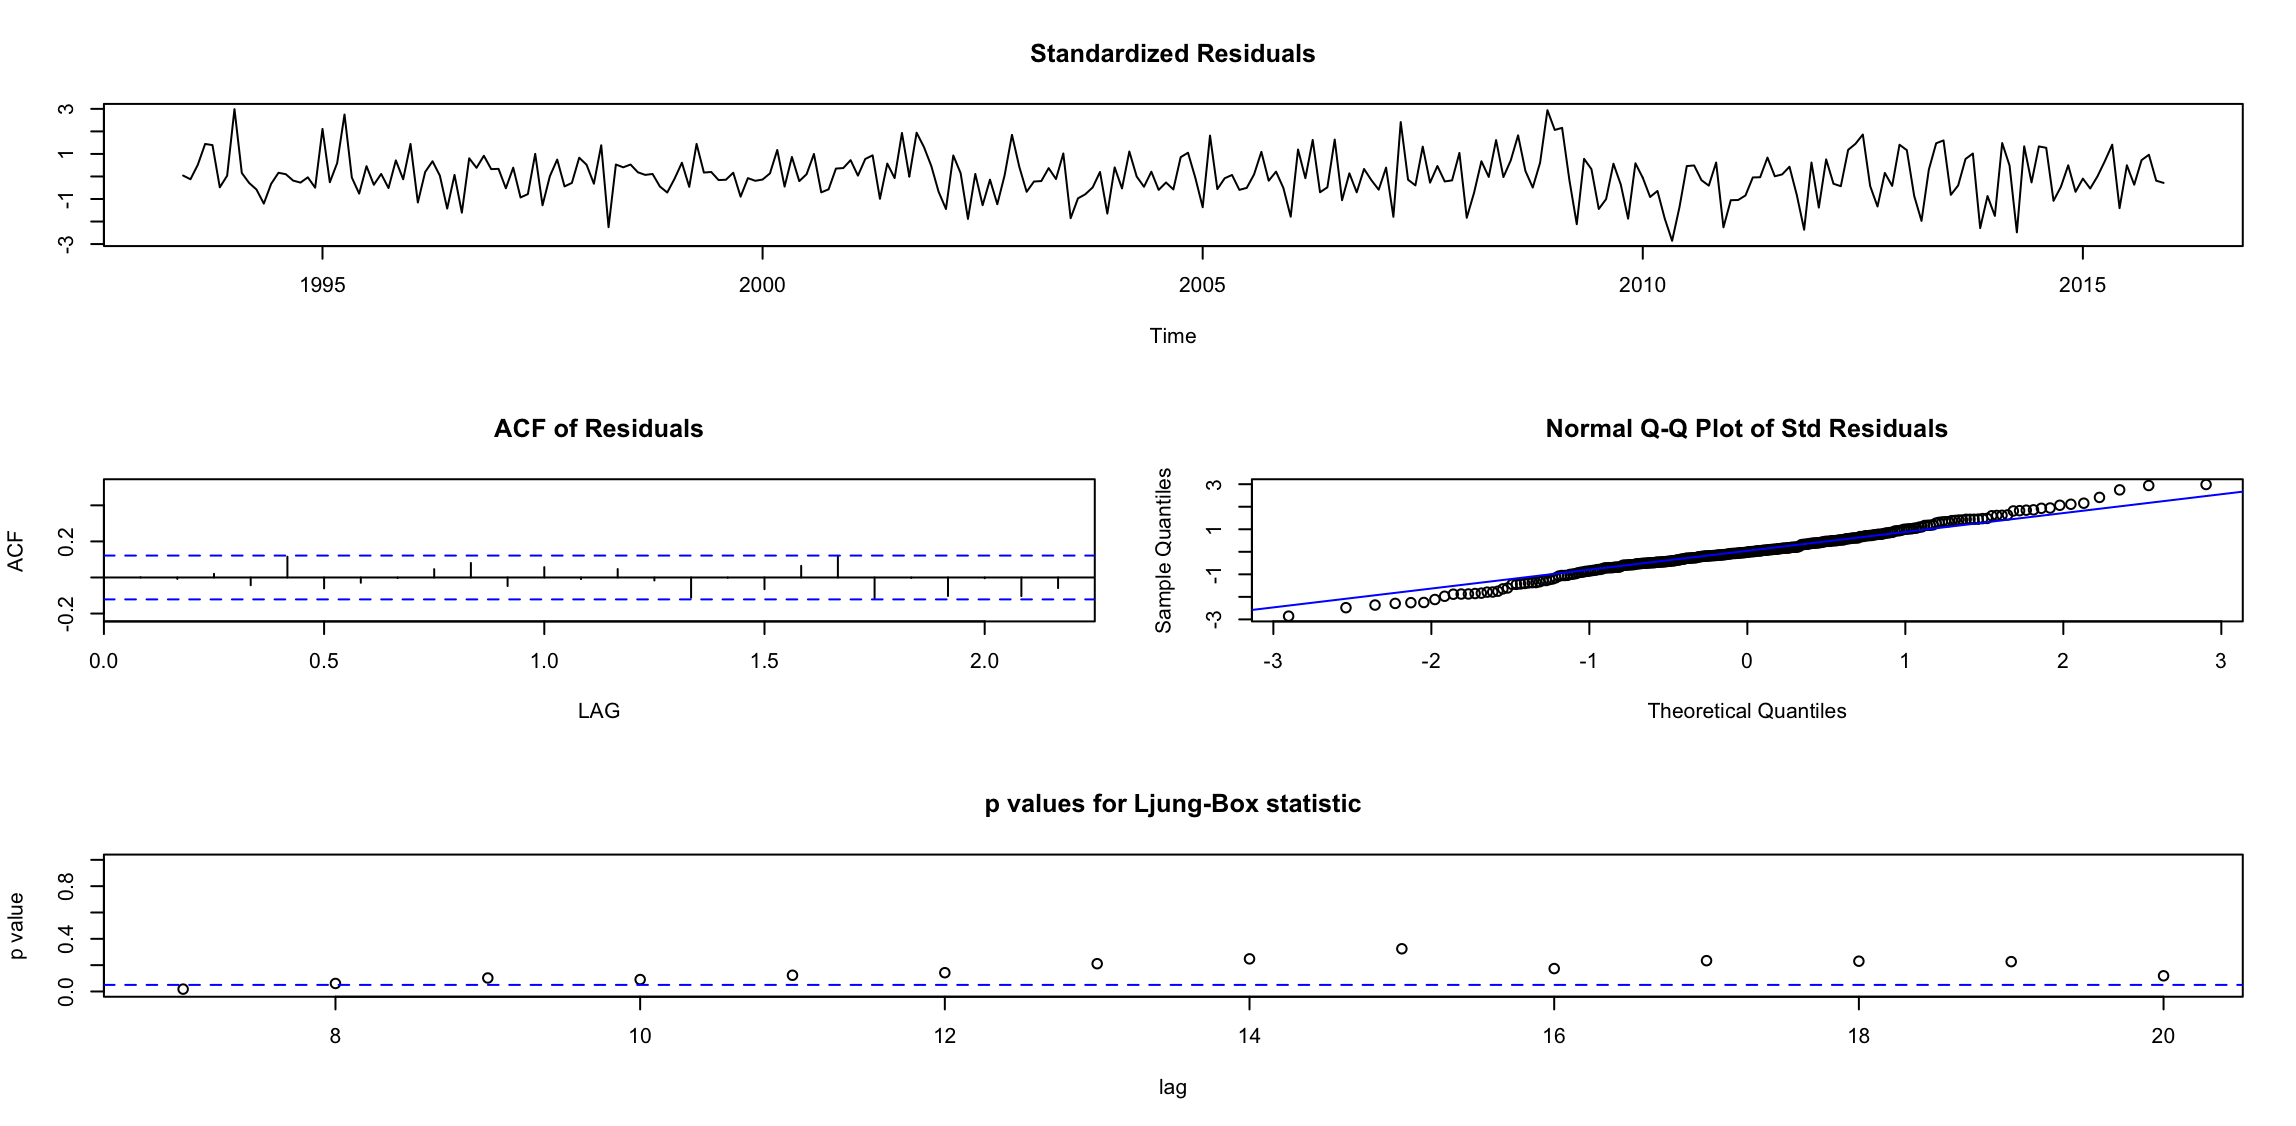
\includegraphics[width=\linewidth]{images/sarima9}
     	\label{fig:sarima9}
      \end{figure}
      

%----------------------------------------------------------------------------------------

\end{document}
